\documentclass[oneside,a4paper,12pt]{article} % Specifies the page format and font size.


% -------------------------------------- Integration of packages --------------------------------------
% Literature and language
\usepackage[english]{babel}
\usepackage{csquotes}
\usepackage[style=apa,backend=biber]{biblatex}
\DeclareLanguageMapping{british}{british-apa}
\addbibresource{Content/bibliography.bib}

% Format and layout
\usepackage[left=3cm,right=3cm,bottom=3cm]{geometry} % Specifies left and right side margins.
\usepackage{setspace} % Package that enables modifying the line spacing.
\setstretch{1.3} % Sets a line spacing of 1.3.
\parindent0pt % Sets the left indent at a new paragraph.
 \parskip10pt % Sets the space between two paragraphs.
\usepackage{footmisc} % Implements a range of footnote options.
\renewcommand{\footnotelayout}{\setstretch{1}} % Sets a line spacing of 1 for the footnotes.
\pagestyle{headings} % Creates a header using the page number and the heading of the current section.
\usepackage{eurosym} % Usage of €

\usepackage{pdflscape}

% Colors
\usepackage{xcolor} % Enables the definition of more colors.

\definecolor{viz-red}{HTML}{FF2C00}
\definecolor{viz-gray}{HTML}{D6DCE5}

\usepackage{colorprofiles} % load colour profiles for pdf/a standard

% https://tex.stackexchange.com/questions/188533/how-to-draw-squares-circles-and-triangles
\usepackage{tikz}
\usetikzlibrary{shapes}

\newcommand{\mysquare}[1]{\tikz{\node[draw=#1,fill=#1,rectangle,minimum
width=0.2cm,minimum height=0.2cm,inner sep=0pt] at (0,0) {};}}

\newcommand{\mycircle}[1]{\tikz{\node[draw=#1,fill=#1,circle,minimum
width=0.2cm,minimum height=0.2cm,inner sep=0pt] at (0,0) {};}}

\newcommand{\mytriangle}[1]{\tikz{\node[draw=#1,fill=#1,isosceles
triangle,isosceles triangle stretches,shape border rotate=90,minimum
width=0.2cm,minimum height=0.2cm,inner sep=0pt] at (0,0) {};}}

% Tables and Graphs
\usepackage{booktabs} % Improves the design of the tables
\usepackage{longtable} % Allows tables to be longer than one page.
\usepackage{threeparttable} % footnotes in tables
\usepackage{multirow,multicol} % With this package it is now possible to combine columns and rows within tables.
\usepackage{graphicx} % Allows to implement graphics.
% \usepackage[font={sf, small}]{subfig} % Enables graphs consisting of several figures.
\usepackage[font={small}]{subfig}
% \usepackage[font={sf, small}]{floatrow} % enables to format tables
\usepackage[font={small}]{floatrow}

\graphicspath{{./Graphs/}} % Tells LATEX that the images are kept in a folder named images under the directory of the main document.
\usepackage[hypcap=false,font={small}]{caption} % Provides many ways to customise captions.
%\usepackage[hypcap=false,font={sf, small}]{caption} % Provides many ways to customise captions.

\usepackage{siunitx} % Enables the use of SI units e. g., proper handling of percentage

% manually define opening bracket which is otherwise parsed by sunitx
% https://tex.stackexchange.com/q/450026/169093
\usepackage{etoolbox} 
\newrobustcmd{\parl}{(}
\newrobustcmd{\parr}{)}

\newcommand*{\tabindent}{ \hspace{2mm}} % Indentation for tables

\sisetup{round-mode=places,round-precision=2, group-separator={,},output-decimal-marker={.}, round-pad = true, input-symbols = {(-)}, % separate-uncertainty=false,
group-minimum-digits=4, % 1,000 instead of 1000
% table-space-text-pre={(},
% table-align-text-pre=false,
% table-space-text-post={$^{***}$},
table-align-text-post=false,
detect-weight=true,
detect-inline-weight=math,
retain-explicit-plus=true,
% round-integer-to-decimal=true,
round-precision=2,
table-format = 1.2, 
} % round to 2 decimal places

\usepackage[super]{nth} % 1st, 2nd etc.
\usepackage{import} % path for inkscape graphics
% Mathematics
 \usepackage{amscd,amsfonts,amsmath,amssymb,amsthm,amscd,bbm} % Extends the maths set.

% PDF/a standard
\usepackage[a-2b,mathxmp]{pdfx}

% Depth
\setcounter{secnumdepth}{3}


% prevent footnotes from being split
% https://texfaq.org/FAQ-splitfoot
\interfootnotelinepenalty=10000


% --------------------------------- Information on thesis ---------------------------------
% Please fill in this information once at the beginning. This way, gaps will be filled in automatically in the following.
\newcommand{\name}{Markus Bilz} % Enter your name.
\newcommand{\dateofthesis}{30 May 2023} % Enter the submission date of your thesis.
\newcommand{\titleofthesis}{Forget About the Rules: Improving Option Trade Classification With Machine Learning} % Enter the title of your thesis.
\newcommand{\streetadress}{Mathystr.~14-16 // XI-11} % Enter your street address.
\newcommand{\postalcode}{76133} % Enter your postal code.
\newcommand{\city}{Karlsruhe} % Enter your city/town.
\newcommand{\email}{markus.bilz@student.kit.edu} % Enter your email address.
\newcommand{\typeofthesis}{Master's Thesis} % specify the type of thesis: Seminar Thesis, Bachelor Thesis, Master Thesis

%--------------------------------- Information in xmpdata ---------------------------------
% definition from macro doesn't seem to work.
\begin{filecontents*}[overwrite]{\jobname.xmpdata}
\Title{Forget About the Rules: Improving Option Trade Classification With Machine Learning}
\Author{Markus Bilz}
\Language{en-GB}
\Keywords{trade-classification\sep machine-learning\sep transformer}
\end{filecontents*}

% --------------------------------- Information in description ---------------------------------
\pdfinfo {
 /Title (\titleofthesis)
 /Author (\name)
 /Subject (Trade Classification using machine learning)
 /Keywords (trade-classification machine-learning transformer) 
}

% --------------------------------- Definition of hyperlinks ---------------------------------
% Hyperreferences
\usepackage{hyperref}
\definecolor{darkblue}{rgb}{0,0,.5}
\hypersetup{
 pdfstartview={FitH},
colorlinks=true,
linkcolor=black,
citecolor=darkblue,
urlcolor=black,
bookmarksopen
}
\usepackage[capitalise, noabbrev]{cleveref} % Enables the use of \cref{} to refer to figures, etc. with Fig.
\creflabelformat{equation}{#2#1#3} % omit round brackets
% https://tex.stackexchange.com/a/121055/169093
\Crefname{appsec}{appendix}{appendices}


\usepackage[symbols,acronyms,automake,savewrites=true,toc,section=section,nopostdot]{glossaries}

\glsaddkey
 {unit}
 {}
 {\glsentryunit}
 {\Glsentryunit}
 {\glsunit}
 {\Glsunit}
 {\GLSunit}

\makeglossaries

% https://tex.stackexchange.com/questions/98494/glossaries-dont-print-single-occurences/230664#230664
\glsenableentrycount % if only used once, dont abbreviate

\newacronym{ANN}{ANN}{artificial neural network}
\newacronym{AUC}{AUC}{area under the curve}
\newacronym{BVC}{BVC}{bulk volume classification}
\newacronym{CRSP}{CRSP}{Center for Research in Securities Prices}
\newacronym{CBOE}{CBOE}{Chicago Board Options Exchange}
\newacronym{CLNV}{CLNV}{Chakrabarty-Li-Nguyen-Van-Ness}
\newacronym{EMO}{EMO}{Ellis-Michaely-O’Hara}
\newacronym{FFN}{FFN}{feed-forward network}
\newacronym{ISE}{ISE}{International Securities Exchange}
\newacronym{GBM}{GBM}{gradient boosting machine}
\newacronym{GSU}{GSU}{Grauer-Schuster-Uhrig-Homburg}
\newacronym{LR}{LR}{Lee-Ready}
\newacronym{MCC}{MCC}{Matthews correlation coefficient}
\newacronym{MLP}{MLP}{multi-layer perceptron}
\newacronym[first={national best bid and offer}]{NBBO}{NBBO}{national best bid and offer}
\newacronym{NYSE}{NYSE}{New York Stock Exchange}
\newacronym{NASDAQ}{NASDAQ}{National Association of Securities Dealers Automated Quotations}
\newacronym{RMSE}{RMSE}{root mean squared error}
\newacronym{RF}{RF}{random forest}
\newacronym{ReLU}{ReLU}{Rectified Linear Units}
\newacronym{SSE}{SSE}{sum of squared errors}
\newacronym{SHAP}{SHAP}{SHapley Additive exPlanations}
\newacronym{TRACE}{TRACE}{Trade Reporting and Compliance Engine}

% see https://tex.stackexchange.com/questions/347586/symbols-as-glossary-entry-indicators
%Symbols
\newglossaryentry{V}{type=symbols,name={\ensuremath{\cong[N_\t{V}]}},sort=V, description={vocabulary}}
\newglossaryentry{A}{type=symbols,name={\ensuremath{A}},sort=A, description={sequence of ask prices}, unit={\ensuremath{=\langle A_{1},A_{2},\dots,A_{T}\rangle}}}
\newglossaryentry{B}{type=symbols,name={\ensuremath{B}},sort=B, description={sequence of bid prices}, unit={\ensuremath{=\langle B_{1},B_{2},\dots,B_{T}\rangle}}}
\newglossaryentry{A-tilde}{type=symbols,name={\ensuremath{\tilde{A}}},sort=A-tilde, description={sequence of ask sizes}, unit={\ensuremath{=\langle \tilde{A}_{1},\tilde{A}_{2},\dots,\tilde{A}_{T}\rangle}}}
\newglossaryentry{B-tilde}{type=symbols,name={\ensuremath{\tilde{B}}},sort=B-tilde, description={sequence of bid sizes}, unit={\ensuremath{=\langle \tilde{B}_{1},\tilde{B}_{2},\dots,\tilde{B}_{T}\rangle}}}
\newglossaryentry{ell}{type=symbols,name={\ensuremath{d_e}}, sort=ell, description={length of token sequence}, unit={\ensuremath{\in \mathbb{N}}}}
\newglossaryentry{e}{type=symbols,name={\ensuremath{\boldsymbol{e}}}, sort=e, description={vector representation / embedding of a token}, unit={\ensuremath{\in \mathbb{R}^{d_e}}}}
\newglossaryentry{d}{type=symbols,name={\ensuremath{d}}, sort=d, description={dimension of a vector}, unit={\ensuremath{\in \mathbb{N}}}}
\newglossaryentry{ellmax}{type=symbols,name={\ensuremath{\ell_{\max}}},sort=ell-max, description={maximum sequence length}, unit={\ensuremath{\in \mathbb{N}}}}
\newglossaryentry{h}{type=symbols,name={\ensuremath{h}},sort=h, description={index of attention heads}}
\newglossaryentry{H}{type=symbols,name={\ensuremath{H}},sort=H, description={number of attention heads}}
\newglossaryentry{P}{type=symbols,name={\ensuremath{P}},sort=p, description={sequence of trade prices}, unit={\ensuremath{=\langle P_{1},P_{2},\dots,P_{T}\rangle}}}
\newglossaryentry{P-tilde}{type=symbols,name={\ensuremath{\tilde{P}}},sort=P-tilde, description={sequence of trade sizes}, unit={\ensuremath{=\langle \tilde{P}_{1},\tilde{P}_{2},\dots,\tilde{P}_{T}\rangle}}}
\newglossaryentry{L}{type=symbols,name={\ensuremath{L}},sort=L, description={number of layers in the encoder / decoder}, unit={\ensuremath{\in \mathbb{N}}}}
\newglossaryentry{M}{type=symbols,name={\ensuremath{M}},sort=m, description={sequence of spread midpoints}, unit={\ensuremath{\langle m_{1},m_{2},\dots,m_{T}\rangle}}}
\newglossaryentry{t}{type=symbols,name={\ensuremath{t}},sort=t, description={index of token in sequence},unit={\ensuremath{\in\left[\ell_{\max }\right]}}}
\newglossaryentry{x}{type=symbols,name={\ensuremath{x}},sort=x, description={primary token sequence}, unit={\ensuremath{\equiv x[1] x[2] \ldots x[\ell] \in V^{\ell}}}}
\newglossaryentry{y}{type=symbols,name={\ensuremath{y}},sort=y, description={trade initiator / target}, unit={\ensuremath{\in \mathcal{Y}}}}
\newglossaryentry{X}{type=symbols,name={\ensuremath{\boldsymbol{X}}},sort=X, description={encoded primary token sequence }, unit={\ensuremath{\in \mathbb{R}^{d_e \times \ell_x}}}}

\newglossaryentry{W-e}{type=symbols,name={\ensuremath{\boldsymbol{W}_e}},sort=W-e, description={token embedding matrix}, unit={\ensuremath{\in \mathbb{R} d_{\mathrm{e}} \times N_{\mathrm{V}}}}}
\newglossaryentry{W-p}{type=symbols,name={\ensuremath{\boldsymbol{W}_p}},sort=W-p, description={positional embedding matrix}, unit={\ensuremath{\in \mathbb{R} d_{\mathrm{e}} \times \ell_{\max}}}}


\newglossarystyle{dotglos}{%
    \setglossarystyle{list}%
    \renewcommand*{\glossentry}[2]{%
        \item[\glsentryitem{##1}\glstarget{##1}{\glossentryname{##1}}]
        \ifglshassymbol{##1}{\glossentrysymbol{##1}}{}%
		\glsentryunit{##1}\quad\parindent20mm%
		\glossentrydesc{##1}%
        \unskip\leaders\hbox to 2.9mm{\hss.}\hfill##2}%
    \renewcommand*{\glsgroupskip}{}%
}

% \renewcommand*{\glossentry}[2]{%
% \item[]\makebox[\glslistdottedwidth][l]{%
% \glsentryitem{##1}%
% \glstarget{##1}{\glossentryname{##1}}%
% \unskip\leaders\hbox to 2.9mm{\hss.}\hfill\strut}\glossentrydesc{##1}}%

% \renewcommand{\glossentry}[2]{%
% \glsentryitem{##1}\glstarget{##1}{\glossentryname{##1}} & $\acem{##1}$ & \glossentrydesc{##1}\tabularnewline
% }%

% 	{\bf Symbol }      \> {\bf Type}     \> {\bf Explanation}                                      \\[0ex]
% 	$[N]$              \> $:=\{1,...,N\}$  \> set of integers $1,2,...,N-1,N$                  \\[0ex]
% 	$i,j$              \> $∈ℕ$           \> generic integer indices       \\[0ex]  
% 	$V$                \> $\cong[N_\t{V}]$      \> vocabulary                               \\[0ex]
% 	$N_\t{V}$          \> $∈\mathbb{N}$  \> vocabulary size                                 \\[0ex]
% 	$V^*$              \> $=\bigcup_{\ell=0}^∞ V^{\ell}$ \> set of token sequences; elements include e.g.\ sentences or documents  \\[0ex]
% 	$\ell_{\max}$      \> $∈\mathbb{N}$     \> maximum sequence length                          \\[0ex]
% 	$\ell$             \> $∈[\ell_{\max}]$      \> length of token sequence                           \\[0ex]  
% 	$t$                \> $∈[\ell]$           \> index of token in a sequence                       \\[0ex]
% 	$d_{...}$          \> $∈ℕ$           \> dimension of various vectors                       \\[0ex]  
% 	$\v{x}$            \> $≡x[1:\ell]$   \> $≡x[1]x[2]...x[\ell]∈V^\ell$ ~~ primary token sequence  \\[0ex]
% 	$\v{z}$            \> $≡z[1:\ell]$   \> $≡z[1]z[2]...z[\ell]∈V^\ell$ ~~ context token sequence  \\[0ex]
% 	$M[i,j]$           \> $∈ℝ$            \> entry $M_{ij}$ of matrix $M∈ℝ^{d×d'}$        \\[0ex]
% 	$M[i,:]\!≡\!M[i]$  \> $∈ℝ^{d'}$      \> $i$-th row of matrix $M∈ℝ^{d×d'}$          \\[0ex]
% 	$M[:,j]$           \> $∈ℝ^d$         \> $j$-th column of matrix $M∈ℝ^{d×d'}$        \\[0ex]
% 	$\v{e}$            \> $∈ℝ^{d_\t{e}}$    \> vector representation / embedding of a token            \\[0ex]
% 	$\m{X}$              \> $∈ℝ^{d_\t{e} × \ell_x}$    \> encoded primary token sequence                             \\[0ex]
% 	$\m{Z}$              \> $∈ℝ^{d_\t{e} × \ell_z}$     \> encoded context token sequence                             \\[0ex]  
% 	$\t{Mask}$         \> $∈ℝ^{\ell_z\times \ell_x}$   \> masking matrix, it determines the attention context for each token \\[0ex]
% 	$L, L_\t{enc}, L_\t{dec}$ \> $∈ℕ$       \> number of network (encoder, decoder) layers                   \\[0ex]  
% 	$l$                \> $∈[L]$           \> index of network layer                             \\[0ex]
% 	$H$                \> $∈\mathbb{N}$     \> number of attention heads                        \\[0ex]
% 	$h$                \> $∈[H]$         \> index of attention head                            \\[0ex]
% 	$N_\t{data}$       \> $∈ℕ$           \> (i.i.d.) sample size                               \\[0ex]  
% 	$n$                \> $∈[N_\t{data}]$     \> index of sample sequence                         \\[0ex]
% 	$η$                \> $∈(0,∞)$           \> learning rate                                      \\[0ex]
% 	$τ$                \> $∈(0,∞)$           \> temperature; it controls the diversity-plausibility trade-off at inference  \\[0ex]
% 	$\m{W_e}$     \> $∈ℝ^{d_\t{e}×N_\t{V}}$ \> token embedding matrix       \\[0ex]  
% 	$\m{W_p}$     \> $∈ℝ^{d_\t{e}×\ell_{\max}}$ \> positional embedding matrix       \\[0ex]  
% 	$\m{W_u}$     \> $∈ℝ^{N_\t{V}×d_\t{e}}$ \> unembedding matrix       \\[0ex]  
% 	$\m{W_q}$     \> $∈ℝ^{d_\t{attn}×d_\t{x}}$ \> query weight matrix \\[0ex]
% 	$\v{b_q}$     \> $∈ℝ^{d_\t{attn}}$ \> query bias \\[0ex]
% 	$\m{W_k}$     \> $∈ℝ^{d_\t{attn}×d_\t{z}}$ \> key weight matrix \\[0ex]
% 	$\v{b_k}$     \> $∈ℝ^{d_\t{attn}}$ \> key bias \\[0ex]
% 	$\m{W_v}$     \> $∈ℝ^{d_\t{out}×d_\t{z}}$ \> value weight matrix \\[0ex]
% 	$\v{b_v}$     \> $∈ℝ^{d_\t{out}}$ \> value bias \\[0ex]
% 	$\bmcWqkv$     \>  \> collection of above parameters of a single-head attention layer \\[0ex]  
% 	$\m{W_o}$     \> $∈ℝ^{d_\t{out}×Hd_\t{mid}}$ \> output weight matrix \\[0ex]
% 	$\v{b_o}$     \> $∈ℝ^{d_\t{out}}$ \> output bias \\[0ex]
% 	$\bmcW$       \>  \> collection of above parameters of a multi-head attention layer, see \cref{eq:Wall} \\[0ex]
% 	$\m{W_\t{mlp}}$    \> $∈ℝ^{d_1×d_2}$ \> weight matrix corresponding to an MLP layer in a Transformer \\[0ex]
% 	$\v{b_\t{mlp}}$    \> $∈ℝ^{d_1}$ \> bias corresponding to an MLP layer in a Transformer \\[0ex]  
% 	$\vga$            \> $∈ℝ^{d_\t{e}}$ \> layer-norm learnable scale parameter \\[0ex]
% 	$\vbe$                \> $∈ℝ^{d_\t{e}}$  \> layer-norm learnable offset parameter \\[0ex]
% 	$\vth,\hat{\vth}$        \> $∈ℝ^d$        \> collection of all learnable / learned Transformer parameters \\[0ex]

%Glossary
\newglossaryentry{activation-function}{name={activation function},plural={activation functions}, description={An activation function is a function, that breaks up the linearity of the neural network. It determines if neurons are activated or not. Common variants include \gls{ReLU} and Softmax.}}
\newglossaryentry{embedding}{name={embedding},plural={embeddings},description={Numerical vector representation of the input, e.g. a word, category, or scalar.}}
\newglossaryentry{feed-forward-network}{name={feed-forward network},plural={feed-forward networks},description={Neural networks without recursion. Well-known variants are \glspl{MLP}.}}
\newglossaryentry{overfitting}{name={overfitting},plural={overfitting},description={Creating a model that fits the training data closely, but does not generalize on unseen data.}}
\newglossaryentry{token}{name={token},plural={tokens},description={Item in a vocabulary. For textual data, tokens can be an individual character, sub-word, a word. 
For tabular data, a token corresponds to a column in the data set.}}
\newglossaryentry{exploding-gradient}{name={exploding gradient},plural={exploding gradients},description={Exploding gradients is a problem encountered in training deep neural networks with backpropagation. Error gradients can accumulate, and result in very large parameter updates and unstable training of the network. The opposite is the vanishing gradient problem, whereby gradients become successively smaller during backpropagation, resulting in no or small parameter updates of the network. In both cases, the network does not converge.}}
% ----------------------------------- Start of document -----------------------------------
\begin{document}
\setcounter{page}{2} % Cover pages and title page are not numbered. Start numbering from page 2.

% Title page
\newgeometry{left=3cm, right=3cm, bottom=2cm}
\begin{titlepage}
		\begin{center}
			{\Large Karlsruhe Institute of Technology \\
			\vspace{0.6cm}
			Institute for Finance\\
			Department of Financial Engineering and Derivatives\\
			Prof. Dr. Marliese Uhrig-Homburg} \\[4.5cm]
			{\large{\typeofthesis}} \\[1.7cm]
			\setstretch{10.0}
			{\Huge {\titleofthesis}}
			\setstretch{1.3} \\[7cm]
		\end{center}
				
		\begin{tabular}{ll}
        Author:     & {\name}\\
                    & {\streetadress}\\
                    & {\postalcode} {\city}\\
					& E-Mail: {\email}\\\\
        Karlsruhe, & {\dateofthesis}\\
    	\end{tabular}
\end{titlepage}
\restoregeometry % Exclude title page (with %) that is not being used.

% Table of contents
\setcounter{page}{1}\renewcommand{\thepage}{\roman{page}} % Sets the numbering to roman small.
\newpage
\tableofcontents

% List of Figures (comment out if there are no figures in the thesis)
\newpage
\listoffigures % Inserts the list of figures.
\addcontentsline{toc}{section}{List of Figures} % Adds the list of figures to the table of contents.

% List of tables (comment out if there are no tables in the thesis)
\newpage
\listoftables % Inserts the list of figures.
\addcontentsline{toc}{section}{List of Tables} % Adds the list of tables to the table of contents.

\newpage
\printglossary[title={List of Symbols},type=symbols,style=dotglos]

% Main text section
\newpage
\setcounter{page}{1}\renewcommand{\thepage}{\arabic{page}} % Sets the numbering to Arabic.

\section{Introduction (2~p)}\label{sec:introduction}

\footnote{The authors acknowledge support by the state of Baden-Württemberg through \href{https://www.bwhpc.de/}{bwHPC}.}
\newpage

\section{Related Work}\label{sec:related-work}

\subsection{Trade Classification in Option Markets}
\label{sec:trade-classification-in-option-markets}

While classical trade classification algorithms are extensively tested in the stock markets (e.g., \textcite[][3806--3821]{chakrabartyTradeClassificationAlgorithms2012}; \textcite[][259--286]{odders-whiteOccurrenceConsequencesInaccurate2000}), few works have examined trade classification in option markets.

\textcite[882--883]{savickasInferringDirectionOption2003} were the first to compare the tick rule, quote rule, the \gls{LR} algorithm and the \gls{EMO} rule for options traded at the \gls{CBOE}. The dataset spans a period from July 3, 1995 -- December 31, 1995 consisting of $869{,}217$ matched trades. The authors report the highest accuracies for the quote rule (\SI{78.98}{\percent}) and find that all rules perform worst when applied to index options. In general, the trade classification rules exhibit significantly lower classification accuracies on options data than with stock data, urging the need for improved classifiers.

The most exhaustive study is the one of \textcite[1--39]{grauerOptionTradeClassification2022}. The authors test the accuracy of the classical quote rule and tick rule, and hybrids thereof on two large-scale datasets spanning a period from 2005 - 2017~\footnote{We formally define accuracy in \cref{sec:evaluation-metric}.}. Consistently for options traded at the \gls{CBOE} and \gls{ISE} classical rules like the popular \gls{LR}  algorithm only achieve accuracies of \SI{62.03}{\percent} or \SI{62.53}{\percent} and are thus significantly smaller than in the stock market. In line with the research of \textcite[886]{savickasInferringDirectionOption2003}, the reported accuracies are inversely proportional to the rule's reliance on past transaction prices. In particular, the tick rule performs worst with accuracies marginally different from a random guess. Overall, the success rates deteriorate between both studies and over time. As a remedy, \textcite[14--17]{grauerOptionTradeClassification2022} introduce two additional rules based on the trade and quote sizes. The depth rule is an alternative to the tick rule for classifying midspread trades in the \gls{LR}  algorithm and \gls{EMO} rule. It assigns the initiator of the trade based on the depth at the bid or ask. Together with the trade size rule, their second rule, which classifies trades with a trade size matching the size of the bid or ask quote, can substantially improve the performance of classical algorithms. The ensemble of rules achieves an accuracy between \SI{73}{\percent} and \SI{75}{\percent} surpassing previous rules by more than \SI{10}{\percent}, at the cost of data efficiency.

The work of \textcite[1--39]{grauerOptionTradeClassification2022} is relevant for two reasons. First, the dataset is identical to ours, which enables a fair comparison between classical rules and machine learning-based predictors. Second, their stacked combinations of the trade size rule, depth rule, and common trade classification algorithms achieve state-of-the-art performance in option trade classification and are thus a rigorous benchmark.

\subsection{Trade Classification Using Machine Learning}
\label{sec:trade-classification-using-machine-learning}

\textcite[5]{rosenthalModelingTradeDirection2012} bridges the gap between classical trade classification and machine learning by fitting a logistic regression model on lagged and unlagged features innate to the tick rule, quote rule, and \gls{EMO} algorithm, as well as a sector-specific and a time-specific term. Instead of using the rule's discretized outcome as a feature, he models the rules through so-called information strength functions \autocite[6--7]{rosenthalModelingTradeDirection2012}. The proximity to the quotes, central to the \gls{EMO} algorithm, is thus modelled by a proximity function. Likewise, the information strength of the quote and tick rule is estimated as the log return between the trade price and the midpoint or the previous trade price. However, it only improves the accuracy of the \gls{EMO} algorithm by a marginal \SI{2.0}{\percent} for \gls{NASDAQ} stocks and \SI{1.1}{\percent} for \gls{NYSE} stocks \autocite[15]{rosenthalModelingTradeDirection2012}. Our work aims to improve the model by exploring non-linear estimators and minimising data modelling assumptions.

The work of \textcite[483]{blazejewskiLocalNonParametricModel2005} compares a $k$-nearest neighbour classifier against logistic regression, as well as simple heuristics like the majority vote over past trades for signing trades at the Australian stock exchange. Their results indicate that the parametric $k$-nearest neighbour classifier improves upon a linear logistic regression in terms of classification accuracy, even when trained on fewer features. The work is unique from the remaining works about the feature set definition. Notably, \textcite[483]{blazejewskiLocalNonParametricModel2005} use no quote or trade prices, but rather the order book volumes, trade sizes, and past trade signs for classification. No accuracies for classical trade signing rules are reported, which impedes a comparison across different works. In line with their results, we focus on non-linear models in the form of gradient boosting and Transformers. Additionally, our paper addresses the mentioned shortcomings by benchmarking against state-of-the-art trade classification rules. We share the idea of using the trade size, as well as the bid and ask sizes for classification for some of our feature sets, but greedily predict using non-historic features.

Closest to our work is a publication by \textcite[1--58]{ronenMachineLearningTrade2022}. Therein, the authors compare a selection of machine learning algorithms against classical trade signing rules in the bond and stock market. Their comparison is the first to consider logistic regression, a random forest, as well as \glspl{feed-forward-network}. Over a wide range of feature sets the tree-based ensemble consistently outperforms by out-of-sample accuracy the tick rule and \gls{LR} algorithm, as well as all remaining machine learning models. For the \gls{TRACE} and ITCH dataset, their best variant of the random forest outperforms the tick rule by \SI{8.3}{\percent} and \SI{3.3}{\percent}, respectively \autocite[57]{ronenMachineLearningTrade2022}. Whilst the superiority of random forests is consistent for the bond and equity market, fitted classifiers do not transfer across markets, as accuracies diminish in a transfer setting.

The results convincingly demonstrate the potential of machine learning, i.e., of tree-based ensembles, for trade classification. Yet, the comparability of the results is limited by the classifier's reliance on additional features beyond quote and price data. Albeit, \textcite[13--14]{ronenMachineLearningTrade2022} consider a wide range of approaches, their selection leaves the latest advancements in artificial neural networks and ensemble learning aside and is mainly guided by computational constraints. Even if the focus is on standard techniques, the unclear research agenda concerning model selection, tuning, and testing hampers the transferability of their results to the yet unstudied option market.

In summary, machine learning has been applied successfully in the context of trade classification. No previous work performs, machine learning-based classification in the options markets.

\newpage
\section{Rule-Based Approaches}\label{sec:rule-based-approaches}

Every option trade has a buyer and seller side. For a plethora of problems in option research, it’s also crucial to determine the party that initiated the transaction.

In the following sections, we provide a concise overview of different trade initiator definitions and present rule-based methods for trade classification.

\subsection{Trade Initiator}
\label{sec:trade-initiator}

Various definitions for the trade initiator have been proposed in prior
research. Among these, the:

\emph{Chronological view:} \textcite[][267]{odders-whiteOccurrenceConsequencesInaccurate2000} adapts a chronological view based on the order arrival. She defines the initiator of the trade as the party (buyer or seller) who places their order last, chronologically. This definition requires knowledge about the order submission times.

\emph{Immediacy view:} In contrast, \textcite[][94--97]{leeInferringInvestorBehavior2000} equate the trade initiator with the party in demand for immediate execution. Thus, traders placing market orders, immediately executable at whatever price, or executable limit orders, are considered the trade initiator. By contrast, the party placing non-executable limit orders, which may not even result in a trade, is the non-initiator. This definition remains ambiguous for trades resulting from crossed limit orders, matched market orders, or batched orders \autocite[][94--95]{leeInferringInvestorBehavior2000}.
% FIXME: introduce of notion of demanding / taking away liquidity and providing liquidity

\emph{Positional view:} Independent from the order type and submission time, \textcite[][533]{ellisAccuracyTradeClassification2000} deduce their definition of the trade initiator based on the position of the involved parties opposite to the market maker or broker. The assumption is, that the market maker or broker only provides liquidity to the investor and the trade would not exist without the initial investor's demand.

The appropriate view differs by data availability and application context.
Regardless of the definition used, the trade initiator is binary and can either be the seller or the buyer. Henceforth, we denote it by $\gls{y} \in \mathcal{Y}$ with $\mathcal{Y}=\{-1,1\}$, with $y=-1$ indicating a seller-initiated and $y=1$ a buyer-initiated trade. The predicted trade initiator is denoted as $\hat{y}$.

As the trade initiator is commonly not provided with the option datasets, it must be inferred using trade classification algorithms \autocite[][453]{easleyOptionVolumeStock1998}. The following section introduces basic rules for trade classification. We start with the ubiquitous quote and tick rule and continue with the more recent depth and trade size rule. Our focus is on classification rules, that sign trades on a trade-by-trade basis. Consequently, we omit classification rules for aggregated trades, like the \gls{BVC} algorithm of \textcite[][1466--1468]{easleyFlowToxicityLiquidity2012}.

\subsection{Basic Rules}\label{sec:basic-rules}

This section presents basic classification rules, that may be used for trade classification independently or integrated into a hybrid algorithm.

\subsubsection{Quote Rule}\label{sec:quote-rule}

The quote rule classifies a trade by comparing the trade price against the corresponding quotes at the time of the trade. We denote the sequence of trade prices of the $i$-th security by $\gls{P}_i = \langle P_{i,1},P_{i,2},\dots,P_{i,T}\rangle$ and the corresponding ask at $t$ by $\gls{A}_{i,t}$ and bid by $\gls{B}_{i,t}$. If the trade price is above the midpoint of the bid-ask spread, estimated as $\gls{M}_{i,t} = \tfrac{1}{2}(B_{i,t} + A_{i,t})$, the trade is classified as a buy and if it is below the midpoint, as a sell \autocite[][41]{harrisDayEndTransactionPrice1989}. Thus, the classification rule on $\mathcal{A} = \left\{(i, t) \in \mathbb{N}^2: P_{i,t} \neq M_{i,t}\right\}$ is given by:

\begin{equation}
    \operatorname{quote}\colon \mathcal{A} \to \mathcal{Y},\quad
    \operatorname{quote}(i, t)=
    \begin{cases}
        1,  & \mathrm{if}\ P_{i, t}>M_{i, t}  \\
        -1, & \mathrm{if}\ P_{i, t}<M_{i, t}. \\
    \end{cases}
\end{equation}

By definition, the quote rule cannot classify trades at the midpoint of the quoted spread. \textcite[][241]{hasbrouckTradesQuotesInventories1988} discusses multiple alternatives for signing midspread trades including ones based on the subsequent quotes, and contemporaneous, or the subsequent transaction. Yet, the most common approach to overcome this limitation is, coupling the quote rule with other approaches, as done in \cref{sec:hybrid-rules}.

The quote rule requires matching one bid and ask quote with each trade based on a timestamp. Due to the finite resolution of the dataset's timestamps and active markets, multiple quote changes can co-occur at the time of the trade, some of which, may logically be after the trade. As such, it remains unclear which quote to consider in trade classification, and a quote timing technique must be employed. Empirically, the most common choice is to use the last quote in the order of the time increment (e.g., second) before the trade \autocite[][1765]{holdenLiquidityMeasurementProblems2014}.

The quote rule depends on price and quote data, which affects the data efficiency. The reduced dependence on past transaction prices and the focus on quotes has nonetheless positively impacted classification accuracies in option markets, as studies of \textcite[][886]{savickasInferringDirectionOption2003} and \textcite[][3]{grauerOptionTradeClassification2022} suggest. Especially, if trade classification is performed on the \gls{NBBO}.


\subsubsection{Tick Test}\label{sec:tick-test}

% TODO: his method uses the previous trade to gauge whether the current trade is at a higher price (and presumably a buy) or at a lower price (and presumably a sell).
A common alternative to the quote rule is the tick test. Based on the rationale that buys increase the trade price and sells lower them, the tick test classifies trades by the change in trade price. It was first applied in \textcites[][244]{holthausenEffectLargeBlock1987}[][240]{hasbrouckTradesQuotesInventories1988}. The tick test is defined as:

\begin{equation}
    \operatorname{tick}\colon \mathbb{N}^2 \to \mathcal{Y},\quad
    \operatorname{tick}(i, t)=
    \begin{cases}
        1,                           & \mathrm{if}\ t=1 \lor P_{t}>P_{t-1} \\
        -1,                          & \mathrm{if}\ P_{i, t} < P_{i, t-1}  \\
        \operatorname{tick}(i, t-1), & \mathrm{else}.
    \end{cases}
    \label{eq:tick-test}
\end{equation}

Considering the cases in \cref{eq:tick-test} the trade price is higher than the previous price (uptick) the trade is classified as a buy~\footnote{To end recursion at $t=1$, we sign the trade to be buyer-initiated to simplify notation. Other choices are possible, e.g., random assignment or based on another rule. Similarly done for \cref{eq:reverse-tick-test}.}. Reversely, if it is below the previous price (downtick), the trade is classified as a sell. If the price change is zero (zero tick), the signing uses the last price different from the current price \autocite[][735]{leeInferringTradeDirection1991}.

By this means, the tick rule can sign all trades as long as a last differing trade price exists, but the overall precision can be impacted by infrequent trading. Being only dependent on transaction data makes the tick rule highly data-efficient. Waiving any quote data for classification contributes to this efficiency, but also poses a major limitation with regard to trades at the bid or ask, as discussed by \textcite[][557--558]{finucaneDirectTestMethods2000}. For instance, if quotes rise between trades, then a sale at the bid on an uptick or zero uptick is misclassified as a buy by the tick test due to the overall increased trade price. Similarly for falling quotes, buys at the ask on downticks or zero downticks are erroneously classified as a sell.


% sometimes dependency on data referred to as level-1 and level-2 (cp. chakrabarty 2015) Level-1 algorithms use only trade price data; level-2 algorithms use both trade and quote data.

The reverse tick test is a variant of the tick test proposed in \textcite[][241]{hasbrouckTradesQuotesInventories1988}. It is similar to the tick rule but classifies based on the next, distinguishable trade price.

\begin{equation}
    \operatorname{rtick} \colon \mathbb{N}^2 \to \mathcal{Y},\quad
    \operatorname{rtick}(i, t)=
    \begin{cases}
        1,                            & \mathrm{if}\ t+1=T \lor P_{i, t} > P_{i, t+1} \\
        -1,                           & \mathrm{if}\ P_{i, t} < P_{i, t+1}            \\
        \operatorname{rtick}(i, t+1), & \mathrm{else}
    \end{cases}
    \label{eq:reverse-tick-test}
\end{equation}

As denoted in \cref{eq:reverse-tick-test}, the trade is classified as seller-initiated, if the next trade is on an uptick or a zero uptick, and classified as buyer-initiated for trades at a downtick or a zero downtick \autocite[][735--636]{leeInferringTradeDirection1991}.

Both tests result in the same classification, if the current trade is bracketed by a price reversal and the price change after the trade is opposite from the change before the trade, but differ for price continuations when price changes are in the same direction \autocite[][736]{leeInferringTradeDirection1991}.

In practice, \textcite[][29--32]{grauerOptionTradeClassification2022} observe higher accuracies for the reverse tick test on a sample of option trades, but both cannot compete with quote-based approaches and calls for more sophisticated approaches.

\subsubsection{Depth Rule}\label{sec:depth-rule}

% TODO: These proxies have in common that they factor in the order book imbalance the relative depth quoted at the best bid and ask prices. If traders care about transaction costs, the relatively wide ask-side spread deters buyers, whereas the tight bid-side spread may attract sellers. There are then more traders submitting market orders at the bid side, and the true effective spread is, on average, smaller than the average midpoint effective spread.
% TODO: Derive in greater detail why orderbook imbalance makes sense! See my notes from Hagströmer

As \cref{sec:quote-rule} unveils, the tick rule yields significantly lower success rates than the quote rule. For midspread trades, that otherwise cannot be classified by the advantageous quote rule, \textcite[][14]{grauerOptionTradeClassification2022} propose the depth rule as an override.

The depth rule gauges the trade initiator from the quoted size at the best bid and ask. Based on the observation that an exceeding bid or ask size relates to higher liquidity at one trade side, trades are classified as a buy (sell) for a larger ask (bid) size \autocite[][14]{grauerOptionTradeClassification2022}.

Let $\gls{A-tilde}_{i,t}$ denote the quoted size of the ask, $\gls{B-tilde}_{i,t}$ of the bid, and $\gls{P-tilde}_{i,t}$ the trade price at $t$ of the $i$-th option. We set the domain as $\mathcal{A} = \left\{(i, t) \in \mathbb{N}^2: P_{i,t} = \gls{M}_{i,t} \land \tilde{A}_{i,t} \neq \tilde{B}_{i,t} \right\}$. The depth rule is now calculated as:
\begin{equation}
    \operatorname{depth} \colon \mathcal{A} \to \mathcal{Y},\quad
    \operatorname{depth}(i, t)=
    \begin{cases}
        1,  & \mathrm{if}\ \tilde{A}_{i,t} > \tilde{B}_{i,t} \land P_{i, t} = M_{i, t}. \\
        -1, & \mathrm{if}\ \tilde{A}_{i,t} < \tilde{B}_{i,t} \land P_{i, t} = M_{i, t}  \\
    \end{cases}
    \label{eq:depth-rule}
\end{equation}

As shown in \cref{eq:depth-rule}, the depth rule classifies midspread trades only, if the ask size is different from the bid size, as the ratio between the ask and bid size is the sole criterion for inferring the trade's initiator. Due to these restrictive conditions in $\mathcal{A}$, the depth rule can sign only a fraction of all trades and must be best stacked with other rules.

Like the quote rule, the depth rule has additional dependencies on quote data. Despite being applied to midpoint trades only, \textcite[][4]{grauerOptionTradeClassification2022} report an improvement in the overall accuracy by \SI{1.2}{\percent} for \gls{CBOE} data and by \SI{0.8}{\percent} for trades from the \gls{ISE} merely through the depth rule. The rule has not yet seen wide adoption.

\subsubsection{Trade Size Rule}\label{sec:trade-size-rule}

% TODO: Think about writing as restriction? https://en.wikipedia.org/wiki/Restriction_(mathematics)
As \cref{sec:tick-test} derives, quote-based approaches are generally preferred due to their stronger performance. \textcite[][13]{grauerOptionTradeClassification2022} stress, however, that the quote rule systematically misclassifies limit orders, and propose an override. On $\mathcal{A} = \left\{(i, t) \in \mathbb{N}^2: \tilde{P}_{i,t} = \tilde{A}_{i,t} \neq \tilde{B}_{i,t} \lor \tilde{P}_{i,t} \neq\tilde{A}_{i,t} = \tilde{B}_{i,t} \right\}$ the trade size rule is defined as:
\begin{equation}
    \operatorname{tsize} \colon \mathcal{A} \to \mathcal{Y},\quad
    \operatorname{tsize}(i, t)=
    \begin{cases}
        1,  & \mathrm{if}\ \tilde{P}_{i, t} = \tilde{B}_{i, t} \neq \tilde{A}_{i, t}  \\
        -1, & \mathrm{if}\ \tilde{P}_{i, t} = \tilde{A}_{i, t} \neq \tilde{B}_{i, t}. \\
    \end{cases}
    \label{eq:trade-size-rule}
\end{equation}

The trade size rule in \cref{eq:trade-size-rule} classifies based on a match between the size of the trade $\tilde{P}_{i, t}$ and the quoted bid and ask sizes. The rationale is, that the market maker tries to fill the limit order of a customer, which results in the trade being executed at the contemporaneous bid or ask, with a trade size equalling the quoted size \autocite[][13]{grauerOptionTradeClassification2022}. When both the size of the ask and bid correspond with the trade size, the result is ambiguous.

\textcite[][13]{grauerOptionTradeClassification2022} obtain an accuracy of \SI{79.92}{\percent} for the subset of option trades at the \gls{ISE} (\SI{22.3}{\percent} of all trades) that can be signed using the methodology, which elevates the performance by \SI{11}{\percent} for the entire sample. Expectedly, the improvement is highest for trades at the quotes and reverses for trades outside the quote \autocite[][15]{grauerOptionTradeClassification2022}. Based on these results, the trade size rule may only be applied selectively to trades inside or at the quote. Since only a fraction of all trades can be classified with the trade size rule, the rule must be combined with other basic or hybrid rules for complete coverage. The subsequent section introduces four hybrid algorithms, that combine basic rules into more sophisticated algorithms.

\subsection{Hybrid Rules}\label{sec:hybrid-rules}

The basic trade classification rules from \cref{sec:basic-rules} can be combined into a hybrid algorithm to enforce universal applicability to all trades and improve the classification performance.


\begin{figure}[ht!]
    \hfill
    \subfloat[\acrshort{LR} Algorithm\label{fig:hybrid-lr}]{
        {\renewcommand\normalsize{\tiny}
                \normalsize
                \input{./Graphs/lr-algo.pdf_tex}}
    }
    \subfloat[\acrshort{EMO} Rule\label{fig:hybrid-emo}]{
        {\renewcommand\normalsize{\tiny}
                \normalsize
                \input{./Graphs/emo-algo.pdf_tex}}
    }
    \subfloat[\acrshort{CLNV} Rule\label{fig:hybrid-clnv}]{
        {\renewcommand\normalsize{\tiny}
                \normalsize
                \input{./Graphs/clnv-algo.pdf_tex}}
    }
    \subfloat[Hybrid Rule Through Stacking\label{fig:hybrid-grauer}]{
        {\renewcommand\normalsize{\tiny}
                \normalsize
                \input{./Graphs/grauer-algo.pdf_tex}}
    }
    \hfill\null
    \caption[Comparison Between Hybrid Trade Classification Rules]{Comparison between hybrid trade classification rules. The Figure visualizes the components of the \acrshort{LR} algorithm, \acrshort{EMO} rule, the \acrshort{CLNV} method, and an arbitrary, stacked combination relative to the quotes. Rules at the midpoint or the quotes are slightly exaggerated for better readability. Own work inspired by \textcite[][167]{poppeSensitivityVPINChoice2016}.}
    \label{fig:hybrid-algorithms}
\end{figure}

Popular variants include the \gls{LR} algorithm, the \gls{EMO} rule, and the \gls{CLNV} method. All three algorithms utilize the quote and tick rule to a varying extent, as depicted in \cref{fig:hybrid-lr,fig:hybrid-emo,fig:hybrid-clnv}. Basic rules are selected based on the proximity of the trade price to the quotes. We study all algorithms in detail in \cref{sec:lee-and-ready-algorithm,sec:ellis-michaely-ohara-rule,sec:chakarabarty-li-nguyen-van-ness-method}.


As put forth by \textcite[][18]{grauerOptionTradeClassification2022}, basic or hybrid rules can be combined through stacking. One such combination is depicted in \cref{fig:hybrid-grauer}. This approach is notably different from the aforementioned algorithms, as the applied rule is no longer dependent on the proximity to the quotes, but rather on the classifiability of the trade with the primary rules and their ordering. We cover this approach last.

\subsubsection{Lee and Ready Algorithm}\label{sec:lee-and-ready-algorithm}

The popular \gls{LR} algorithm \autocite[][745]{leeInferringTradeDirection1991} combines the (reverse) tick test and quote rule into a single rule, which is derived from two observations. First, \textcite[][735--743]{leeInferringTradeDirection1991} observe a higher precision of the quote rule over the tick rule, which makes it their preferred choice. Second, by the means of a simple model, the authors demonstrate that the tick test can correctly classify at least \SI{85.0}{\percent} of all midspread trades if the model's assumptions of constant quotes between trades and the arrival of the market and standing orders following a Poisson process are met.

In combination, the algorithm primarily signs trades according to the quote rule. Trades at the midpoint of the spread, unclassifiable by the quote rule, are classified by the tick rule. Overall:

\begin{equation}
    \operatorname{lr} \colon \mathbb{N}^2 \to \mathcal{Y},\quad\operatorname{lr}(i,t)=
    \begin{cases}
        1,                         & \mathrm{if}\ P_{i, t} > M_{i, t} \\
        -1,                        & \mathrm{if}\ P_{i, t} < M_{i, t} \\
        \operatorname{tick}(i, t), & \mathrm{else}.
    \end{cases}
\end{equation}

As the algorithm requires both trade and quote data, it is less data-efficient than its subparts. Even if data is readily available, in past option studies the algorithm does not significantly outperform the quote rule and outside the model's tight assumptions the expected accuracy of the tick test is unmet \autocites[][30--32]{grauerOptionTradeClassification2022}[][886]{savickasInferringDirectionOption2003}. Nevertheless, the algorithm is a common choice in option research \autocite[cp.][453]{easleyOptionVolumeStock1998}. It is also the basis for more advanced algorithms, such as the \gls{EMO} rule, which we cover next.

\subsubsection{Ellis-Michaely-O'Hara
    Rule}\label{sec:ellis-michaely-ohara-rule}

\textcite[][536]{ellisAccuracyTradeClassification2000} examine the performance of the previous algorithms for stocks traded at \gls{NASDAQ}. By analysing miss-classified trades with regard to the proximity of the trade to the quotes, they observe, that the quote rule and by extension, the \gls{LR} algorithm, perform particularly well at classifying trades executed at the bid and the ask price but trail the performance of the tick rule for trades inside or outside the spread \autocite[][535--536]{ellisAccuracyTradeClassification2000}. The authors combine these observations into a single rule, known as the \gls{EMO} algorithm.

As such, the \gls{EMO} algorithm extends the tick rule by classifying trades at the quotes using the quote rule, and all other trades with the tick test. Formally, the classification rule is given by:
\begin{equation}
    \operatorname{emo} \colon \mathbb{N}^2 \to \mathcal{Y}, \quad
    \operatorname{emo}(i, t)=
    \begin{cases}
        1,                         & \mathrm{if}\ P_{i, t} = A_{i, t} \\
        -1,                        & \mathrm{if}\ P_{i, t} = B_{i, t} \\
        \operatorname{tick}(i, t), & \mathrm{else}.
    \end{cases}
    \label{eq:emo-rule}
\end{equation}

\Cref{eq:emo-rule} embeds both the quote and tick rule. As trades off the quotes are classified by the tick rule, the algorithm's overall success rate is dominated by the tick test assuming most trades are off-the-quotes. For option markets \autocites[cp.][891]{savickasInferringDirectionOption2003}[][21]{grauerOptionTradeClassification2022} this dependence causes the performance to lag behind quote-based approaches, contrary to the successful adaption in the stock market \autocites[][541]{ellisAccuracyTradeClassification2000}[][3818]{chakrabartyTradeClassificationAlgorithms2007}. \textcite[][31--35]{grauerOptionTradeClassification2022} improve the classification accuracy for option trades by applying the reverse tick test as a proxy for the tick test.

\subsubsection{Chakrabarty-Li-Nguyen-Van-Ness
    Method}\label{sec:chakarabarty-li-nguyen-van-ness-method}

Like the previous two algorithms, the \gls{CLNV} method of \textcite[][3809]{chakrabartyTradeClassificationAlgorithms2012} is a hybrid of the quote and tick rule and extends the \gls{EMO} rule by a differentiated treatment of trades inside the quotes, which are notoriously hard to classify. The authors segment the bid-ask spread into deciles (ten equal-width bins) and classify trades around the midpoint (\nth{4} to \nth{7} decile) by the tick rule and trades close or outside the quotes are categorized by the tick rule.

\begin{equation}
    \operatorname{clnv} \colon \mathbb{N}^2 \to \mathcal{Y}, \quad
    \operatorname{clnv}(i, t)=
    \begin{cases}
        1,                         & \mathrm{if}\ P_{i, t} \in \left(\frac{3}{10} B_{i,t} + \frac{7}{10} A_{i,t}, A_{i, t}\right] \\
        -1,                        & \mathrm{if}\ P_{i, t} \in \left[ B_{i,t}, \frac{7}{10} B_{i,t} + \frac{3}{10} A_{i,t}\right) \\
        \operatorname{tick}(i, t), & \mathrm{else}
    \end{cases}
    \label{eq:CLNV-rule}
\end{equation}

% TODO: sucess rates are sensitive to trade location.

The algorithm is summarized in \cref{eq:CLNV-rule}. It is derived from a performance comparison of the tick rule (\gls{EMO} rule) against the quote rule (\gls{LR} algorithm) on stock data, whereby the accuracy was assessed separately for each decile \footnote{The spread is assumed to be positive and evenly divided into ten deciles and the \nth{1} to \nth{3} deciles are classified by the quote rule. Counted from the bid, the \nth{1} decile starts at $B_{i,t}$ and ends at $B_{i,t} + \tfrac{3}{10} (A_{i,t} - B_{i,t}) = \tfrac{7}{10} B_{i,t} + \tfrac{3}{10} A_{i,t}$ \nth{3} decile. As all trade prices are below the midpoint, they are classified as a sell.}. The classical \gls{CLNV} method uses the backward-looking tick rule. In the spirit of \textcite[][735]{leeInferringTradeDirection1991}, the tick test could be exchanged for the reverse tick test.

\subsubsection{Stacked Rule}\label{sec:stacked-rule}

The previous algorithms are static concerning the used base rules and their alignment. Combining arbitrary rules into a single algorithm requires a generic procedure. \textcite[][18]{grauerOptionTradeClassification2022} combine basic and hybrid rules through stacking. In this setting, the trade traverses a stack of pre-defined rules until a rule can classify the trade or the end of the stack is reached~\footnote{For a trade, which cannot be classified by any classifier, one may fallback on a random assignment or the majority class if the distribution of trades is imbalanced.}. The classification is now dependent on the employed rules but also on their ordering.

% TODO: Murjajev (quote + quote on nbbo)
The most basic application is in the \gls{LR} algorithm. For a more complex example consider the hybrid rule consisting of $\operatorname{tsize} \to \operatorname{quote} \to \operatorname{tick}$ in \cref{fig:stacking-algo}. An exemplary trade cannot be classified by the primary trade size rule and is signed by the quote rule, which is the first rule in the stack, able to classify the trade. Other trades can be classifiable by the trade size rule, which rules out the classification of the quote and tick rule. Theoretically, stacked rules can grow to great depth with an arbitrary arrangement. In practice, rules may be ordered greedily and new rules added if there are unclassified trades.

\begin{figure}[ht!]
    \centering
    \input{./Graphs/stacking-algo.pdf_tex}
    \caption[Stacked Trade Classification Rules]{Stacked rule consisting of the trade size (first) and quote rule (second) as well the tick test (third). Coloured shapes indicate the domain of the base rules in a modified scale. The trade is not classifiable by the trade size rule, as indicated by the arrows outside the rule's domain. The quote rule is applied, as it is the first rule to classify the trade entirely. Own drawing.}
    \label{fig:stacking-algo}
\end{figure}

\textcite[][3811]{chakrabartyTradeClassificationAlgorithms2007} and \textcite[][18]{grauerOptionTradeClassification2022} continue the trend for more complex classification rules, leading to a higher fragmented decision surface, and eventually resulting in improved classification accuracy. Since the condition, for the selection of the base rule, is inferred from \emph{static} cut-off points at the decile boundaries of the spread including the midspread and the quotes. Hence, current classification rules may not unleash their full potential. A obvious question is, if classifiers, \emph{learned} on price and quote data, can adapt to the data and thereby improve over classical trade classification rules.

The trend towards sophisticated, hybrid rules, combining as many as five base rules into a single classifier \autocite[cp.][18]{grauerOptionTradeClassification2022}, has conceptual parallels to stacked ensembles found in machine learning and expresses the need for better classifiers.

We provide an overview of state-of-the-art machine learning-based classifiers and start by framing trade classification as a supervised learning
problem.

% In order to evaluate how much prediction models rely on variables, we now introduce notation for random variables, data, classes of prediction models, and loss functions for evaluating predictions.

\newpage
\addtocontents{toc}{\protect\newpage}
\section{Supervised Approaches}\label{sec:supervised-approaches}

% TODO: central assumption of supervised learning (smoothness assumption) (p. 5 chapelle)

\subsection{Framing as a Supervised Learning Problem}\label{sec:problem-framing}

All presented trade classification rules from \cref{sec:rule-based-approaches}  perform \emph{discrete classification} and assign a class to the trade. Naturally, a more powerful insight is to not just obtain the most probable class, but also the associated class probabilities for a trade to be a buy or sell. This gives additional insights into the confidence of the prediction.

Thus, we frame trade signing as a supervised, probabilistic classification task. This is similar to \textcite[][272]{easleyDiscerningInformationTrade2016}, who alter the tick rule and \gls{BVC} algorithm to obtain the probability estimates of a buy from an individual or aggregated trades, but with a sole focus on trade signing on a trade-by-trade basis. A probabilistic view enables a richer evaluation, but constraints our selection to probabilistic classifiers. For comparability, classical trade signing rules need to be modified to yield both the predicted class (buy or sell) and the associated class probabilities.

We introduce more notation, which we use throughout. Each data instance consists of a feature vector and the target. The former is given by $\mathbf{x} \in \mathbb{R}^{1 \times M}$ and described by a random variable $X$. Any of the $M$ features in $\mathbf{x}$ may be numerical, e.g., the trade price or categorical e.g., the option type. Like before, the target is given by $y \in \mathcal{Y}$ and described by a random variable $Y$. Each data instance is sampled from a joint probability distribution $\Pr(X, Y)$. The labelled data set with $N$ i.i.d. samples is denoted by $\mathcal{S} =\left\{\left(\mathbf{x}_i, y_i\right)\right\}_{i=1}^N$. For convienience, we define a feature matrix $\mathbf{X}=\left[\mathbf{x}_1,\ldots, \mathbf{x}_N\right]^{\top}$, that stores all instances and a corresponding vector of labels $\mathbf{y}=\left[y_1,\ldots, y_N \right]^{\top}$.

For our machine learning classifiers, we aim to model $\Pr_{\theta}(y \mid \mathbf{x})$ by fitting a classifier with the parameters $\theta$ on the training set. As classical trade classification rules produce no probability estimates, we use a simple classifier instead:

\begin{equation}
    \widehat{\operatorname{Pr}}(y\mid \mathbf{x})= \begin{cases}1, & \text { if } y=\hat{y} \\ 0, & \text { else }.\end{cases}
    \label{eq:prob-from-point-estimate}
\end{equation}

% TODO: It's actually a one-hot vector with the "probabilities
Consequently, if a trade is predicted as a sell, hence $\hat{y} = -1$, we assign a probability of one for being a sell and a zero probability for being a buy and vice versa. Given the estimated class probabilities, we retrieve the most probable class in $\mathcal{Y}$ as:
\begin{equation}
    \hat{y}=\arg\max_{y \in \mathcal{Y}} \widehat{\operatorname{Pr}}(y \mid \mathbf{x}).
    \label{eq:class-from-prob}
\end{equation}
\cref{eq:prob-from-point-estimate} and \cref{eq:class-from-prob} allow to alternate between a discrete and probabilistic formulation for trade classification rules. Since the class probability estimates are either 0
and 1, no insight into the confidence of the prediction is gained. Nonetheless, this approach enables a seamless comparison of classical rules and probabilistic classifiers in machine learning. Next, we discusses state-of-the-art classifiers suitable for trade classification.

\subsection{Selection of Approaches (2~p)}\label{sec:selection-of-approaches}

\textbf{TODO:} Add a short discussion here, that derives why gradient boosting and Transformers should be used.

\subsection{Gradient Boosted Trees}\label{sec:gradient-boosted-trees}

\subsubsection{Decision Tree}\label{sec:decision-tree}

Decision trees can be used in classification and regression. Despite solving a classification task, our focus is solely on regression trees, as it is the prevailing prediction model used in the gradient boosting algorithm \autocite[][9]{friedmanAdditiveLogisticRegression2000}. For this section, assume $y_i \in \mathbb{R}$.

A decision tree splits the feature space into several disjoint regions $R$ through a sequence of recursive splits. For a binary decision tree, a single split leads to two new sub-regions, whose shape is determined by the features considered for splitting and the preceding splits. Trees are grown in depth until a minimum threshold for the number of samples within a node or some other stopping criterion applies \autocite[][42]{breimanClassificationRegressionTrees2017}.
A region corresponds to a terminal node in the tree. For each terminal node of the tree or unsplit region, the predicted response value is constant for the entire region and shared by all its samples \autocite[][229]{breimanClassificationRegressionTrees2017}.

For a tree with $J$ regions $R_1, R_2,\ldots, R_J$, and some numerical input $\mathbf{x}$ the tree can be modelled as:
\begin{equation}
    h(\mathbf{x})=\sum_{j=1}^{J} \gamma_{j} \mathbb{I}\left(\mathbf{x} \in R_{j}\right),
    \label{eq:decision-tree}
\end{equation}

where $\mathbb{I}$ is the indicator function for region conformance and $\gamma_j$ the region's constant \autocite[][326]{hastietrevorElementsStatisticalLearning2009}. In the regression case, $\gamma_j$ is the mean of all target variables $y_i$ in the specific region. Since all samples of a region share a common response value, the tree estimates resemble a histogram that approximates the true regression surface.

So far, it remains open how the best split can be found. The best split is where the deviation between the prediction and the true response variable diminishes. For a single region, this error can be captured in the \gls{SSE} given by:
\begin{equation}
    \operatorname{L}_{\mathrm{SSE}} =\sum_{\mathbf{x}_{i} \in R_j}\left(y_{i}-\gamma_{j}\right)^{2},
\end{equation}

which is subsequently minimised \textcite[][231]{breimanClassificationRegressionTrees2017}. As documented in \textcite[][326]{hastietrevorElementsStatisticalLearning2009} we start with the entire dataset and scan through all combinations of features and possible split values. For a split by the feature $k$ at the value $s$, the child nodes are given by a pair of half-planes:

\begin{equation}
    R_1(k, s)=\left\{X \mid X_k \leq s\right\} \text { and } R_2(k, s)=\left\{X \mid X_k>s\right\}.
\end{equation}

Thereby, the feature $k$ and value $s$ are selected in a way, that the squared error in the child nodes is minimised:
\begin{equation}
    \min _{k, s}\left[\min _{\gamma_1} \sum_{\mathbf{x}_i \in R_1(k, s)}\left(y_i-\gamma_1\right)^2+\min _{\gamma_2} \sum_{\mathbf{x}_i \in R_2(k, s)}\left(y_i-\gamma_2\right)^2\right].
\end{equation}

Trivially, growing deeper trees leads to an improvement in the \gls{SSE}. Considering the extreme, where each sample has its region, the tree would achieve a perfect fit in-sample but perform poorly on out-of-sample data. To reduce the sensitivity of the tree to changes in the training data, hence \emph{variance}, size complexity pruning procedures are employed. Likewise, if the decision tree is too simplistic, a high bias contributes to the model's overall expected error. Both extremes are to be avoided.

Ensemble methods, such as \emph{bagging} \autocite[][123]{breimanBaggingPredictors1996} and \emph{boosting} \autocite[][197--227]{schapireStrengthWeakLearnability1990}, decrease the expected error of the decision tree by combining multiple trees in a single model. Both approaches differ in the error term being minimised, which is reflected in the training procedure and the complexity of the ensemble members. More specifically, bagging decreases the variance, whereas boosting addresses the bias and variance \autocites[][1672]{schapireBoostingMarginNew1998}[][29]{breimanRandomForests2001}. Next, we focus on \gls{GBM}, a variant of boosting.

\subsubsection{Gradient Boosting
    Procedure}\label{sec:gradient-boosting-procedure}

% Gradient boosting iteratively combines oversimplified models, the weak learners, into an additive model to obtain an improved ensemble estimate. This chapter draws on \textcite[][9]{friedmanGreedyFunctionApproximation2001} to derive gradient boosting for binary classification.

% % classifier with outputs in [-1, 1]
% By \cref{sec:problem-framing} we perform binary probabilistic classification and by \cref{sec:trade-initiator} we defined the labels to be $y \in \{-1,1\}$. For gradient boosting, instead of modelling the class-conditional probabilities directly, we model the conditional log odds instead, which can be interpreted as the probability of observing class $1$ or a buyer-initiated trade, and covert to class-conditional probabilities as needed.

% Following \textcite[][9]{friedmanStochasticGradientBoosting2002} we set the loss function to be the cross-entropy loss, given by:

% \begin{equation}
%     L_{\mathrm{CE}} \colon \mathbb{R}^2 \to \mathbb{R} \quad L_{\mathrm{CE}}(y, F) = \log(1+\exp(-2yF))
%     \label{eq:cross-entropy-loss}
% \end{equation}

% where:
% \begin{equation}
%     F(\mathbf{x}) = \frac{1}{2} \log \left[\frac{\Pr(y=1\mid \mathbf{x})}{\Pr(y=-1\mid \mathbf{x})}\right]
%     \label{eq:logits-gbm}
% \end{equation}
% $F(\mathbf{x})$ is the model's prediction in terms of conditional log-odds. The cross-entropy loss, is a reasonable choice, as it is suitable for binary classification, convex, and twice differentiable: properties we exploit later.

% We first intialise the model with a naïve prediction, based on the average class $\bar{y}$ from all training samples:

% \begin{equation}
%     F_0(\mathbf{x})= \frac{1}{2} \log \left[\frac{1+\bar{y}}{1-\bar{y}}\right].
% \end{equation}
% Expectedly, $F_0(\mathbf{x})$ is a poor estimate, capturing hardly any regularities of the data. Gradient boosting solves this issue by adding weak learners to the ensemble. New trees are added greedily, one per iteration $m$ with $m=1,2,\cdots M$. The weak learner in the $m$-th iteration is chosen to approximate the pseudo residual $r_i$, which is the negative gradient of the observed value of the $i$-th sample and the current estimate:

% \begin{equation}
%     r_i=-\left[\frac{\partial L_{\mathrm{CM}}\left(y_i, F\left(\mathbf{x}_i\right)\right)}{\partial F\left(\mathbf{x}_i\right)}\right]_{F(\mathbf{x})=F_{m-1}(\mathbf{x})}=2 y_i /\left(1+\exp \left(2 y_i F_{m-1}\left(\mathbf{x}_i\right)\right)\right).
% \end{equation}

% % TODO: yields the maximum decrease are similar to the components of the negative gradient descent. However, the  major drawback is tha tthe gradient is only defined for data points x_i seen during training, contradicting the creation of a generalising model. 

% Typically, regression trees (cp. \cref{sec:decision-tree}) are chosen as weak learners since they are computationally cheap and can produce continuous estimates for the residual. The $m$-th regression tree contains $J$ terminal regions, denoted by $R_{j m}, j=1,2, \ldots, J_{m}$. We search for an estimate $\gamma_{j,m}$ for the terminal node $R_{jm}$ that minimizes the cross-entropy over all samples within the node:

% \begin{equation}
%     \gamma_{j m}=\arg \min _\gamma \sum_{\mathbf{x}_i \in R_{j m}} \log \left(1+\exp \left(-2 y_i\left(F_{m-1}\left(\mathbf{x}_i\right)+\gamma\right)\right)\right)
%     \label{eq:region-estimate-gbm}
% \end{equation}
% % TODO: Fill in footnote
% \cref{eq:region-estimate-gbm} cannot be solved in closed form and is typically approached by the Newton-Raphson method with a second-order approximation of the loss~\footnote{Compare the second-order Taylor polynomial given by (...).}:

% \begin{equation}
%     \gamma_{j m}=\sum_{\mathbf{x}_i \in R_{j m}} r_i / \sum_{\mathbf{x}_i \in R_{j m}}\left|r_i\right|\left(2-\left|r_i\right|\right)
% \end{equation}
% with $r_i$ given by \cref{eq:logits-gbm}.

% An improved estimate for $\mathbf{x}$ is calculated from the previous estimate by adding the new regression tree to the ensemble. The latter moves the prediction towards the greatest descent and thus improves the overall prediction. The updated model is given by:

% \begin{equation}
%     F_{m}(\mathbf{x})=F_{m-1}(\mathbf{x})+\eta \sum_{j=1}^{J_{m}} \gamma_{j m} \mathbb{I}\left(\mathbf{x} \in R_{j m}\right).
% \end{equation}
% After $M$ iterations we obtain the final estimate calculated as $F_M(\mathbf{x})$. To avoid \gls{overfitting} the residuals, only proportional steps towards the negative gradient are taken, which is controlled by the learning rate $\eta \in \left(0, 1\right]$ \autocite[][13]{friedmanGreedyFunctionApproximation2001}. The learning rate $\eta$ and the size of the ensemble $M$ are deeply intertwined are best tuned together \autocite[][13]{friedmanGreedyFunctionApproximation2001}.

% Gradient boosting is still prone to \gls{overfitting}. One solution is to employ early stopping, whereby the ensemble is only grown in size, as long as adding more weak learners leads to a decrease in loss on the validation set \autocite[][384]{hastietrevorElementsStatisticalLearning2009}. Another approach is to limit the amount of data seen during training by fitting trees on random subset of samples, as proposed in \textcite[][3]{friedmanStochasticGradientBoosting2002}, or on a subset of features, as popularized by \textcite[][3]{chenXGBoostScalableTree2016}. \textcite[][6]{prokhorenkovaCatBoostUnbiasedBoosting2018} grow oblivious trees, which use the same splitting criterion for all nodes of one level in a tree. The rationale is, that these arguably simplistic trees, and achieve an imperfect fit, which regularises the model. Finally, the loss function can be extended for a $\ell_2$ regularization term to penalize the model for complexity, as applied in \textcite[][2]{chenXGBoostScalableTree2016}.

% In recent years, several variants of gradient boosting have been proposed and studied in the literature, including \emph{CatBoost} \autocite[][1--23]{prokhorenkovaCatBoostUnbiasedBoosting2018}, \emph{XGBoost} \autocite[][1--13]{chenXGBoostScalableTree2016}, and \emph{XGBoost} \autocite[][1--13]{chenXGBoostScalableTree2016}, which differ by the policy how trees are grown and how \gls{overfitting} is addressed. Performance-wise, differences between the implementations are negligible, as empirical studies suggest \autocites[cp.][8]{grinsztajnWhyTreebasedModels2022}[][19--20]{gorishniyRevisitingDeepLearning2021}[][7]{somepalliSaintImprovedNeural2021}.

% As we noted at the beginning, $F_M(\mathbf{x})$ models the log odds. We can recover the class-conditional probabilities $\widehat{\operatorname{Pr}}(y \mid \mathbf{x})$ by taking the inverse:

% \begin{equation}
%     \widehat{\operatorname{Pr}}(y \mid \mathbf{x}) = 1 /\left(1+\exp(-2yF_M(\mathbf{x}))\right).
% \end{equation}
% and get the majority class by \cref{eq:class-from-prob}.

\subsection{Transformer Networks}\label{sec:transformer-networks}

The subsequent chapters provide an introduction to classifiers based on the Transformer architecture.

\subsubsection{Architectural Overview}\label{sec:architectural-overview}

The Transformer is a neural network architecture by \textcite[][2--6]{vaswaniAttentionAllYou2017} proposed for sequence-to-sequence modelling. Its original application is in machine translation, whereby sentences in the source language are translated into sentences in the target language. More precisely, the sentence is first decomposed into individual \glspl{token} and mapped into a sequence of \glspl{embedding}, which are rich vector representations of the raw input. The Transformer then processes the \glspl{embedding} to generate the output sequence.

As the network operates on \glspl{embedding}, rather than strings, the architecture is not constrained to process textual data. It has been adapted to other representations including image data \autocites[][2--5]{parmarImageTransformer2018}[][3]{dosovitskiyImageWorth16x162021} and tabular data \autocite[cp.][18932]{gorishniyRevisitingDeepLearning2021}. The latter is important for our work, as derived in \cref{sec:selection-of-approaches}.

Following the architecture for machine translation of \textcite[][3]{sutskeverSequenceSequenceLearning2014}, the network features two main components: the encoder and the decoder. A sequence of \glspl{token} is first mapped to a sequence of \glspl{embedding} and augmented with positional information. The encoder receives these \glspl{embedding} and creates an enriched representation from it by encoding the context in which the input appears i.e., the surrounding words. The output of the encoder is then fed to the decoder. The decoder takes the embedded target sequence along with parts of the encoded representation of the input, to autoregressively generate the output sequence, i.e., the translation in the target language \gls{token} by \gls{token} \autocite[][3]{vaswaniAttentionAllYou2017}. \cref{fig:transformer-architecture-overview} depicts the complete architecture and serves as a guide through the subsequent sub-chapters.

The encoder consists of $\gls{L}=6$ stacked Transformer blocks \autocite[][6]{vaswaniAttentionAllYou2017}. Each block itself is composed of two sublayers: a multi-head self-attention layer, followed by a position-wise, \gls{feed-forward-network}. Both components serve a distinct purpose in the Transformer. The self-attention mechanism encodes the context in which the input appears onto the \glspl{embedding}, whereas the \gls{feed-forward-network} serves as a long-term memory persisting information outside the immediate context. In the multi-head self-attention mechanism of the encoder, inputs can learn from any \gls{token} of the input sequence, even if a \gls{token} appears causally before the other input. Each of the sublayers is surrounded by skip connections \autocite[][2]{heDeepResidualLearning2015} and followed by layer normalization \autocite[][4]{baLayerNormalization2016} to facilitate and stabilize training. Stacking multiple Transformer blocks enables the model to learn hierarchical features from the inputs and targets. Applied to language processing, the first layers in the stack extract coarse-grained syntactic features, and subsequent layers learn fine-grained semantic features \autocites[][3651]{jawaharWhatDoesBERT2019}[][4596]{tenneyBERTRediscoversClassical2019}. For tabular data, this translates to frequent feature combinations or infrequent feature interactions.

Aside from the feed-forward sublayer, the decoder contains a sublayer for multi-head self-attention on the output of the encoder, known as cross-attention, and a masked variant of the multi-head self-attention for use on the output sequence. Here, causal masking enforces the autoregressive properties of the decoder.

%TODO: Graphics contains a typo: W_q in cross attention comes from output sequence. Also fonts are wrong. They should be mathbf. rename to cross-attention?
\begin{landscape}
    \begin{figure}[ht]
        \centering
        {\renewcommand\normalsize{\scriptsize}%
            \normalsize
            \input{./Graphs/transformer-architecture.pdf_tex}}
        \caption[Overview Over the Transformer Architecture]{Overview Over the Transformer Architecture. The left part shows the self-attention mechanism discussed in \cref{sec:attention}. The central part depicts the multi-head self-attention mechanism, as covered in \cref{sec:attention}. The right part shows the encoder and decoder stack, as well as the \gls{embedding} mechanism as covered in \cref{sec:token-embeddings} onwards. Own work inspired by \textcite[][3]{tayEfficientTransformersSurvey2022}.}
        \label{fig:transformer-architecture-overview}
    \end{figure}
\end{landscape}
The output of the decoder is finally passed through a linear layer with a softmax activation function to unembed the output and retrieve the probabilities of the next \gls{token} \autocite[][5]{vaswaniAttentionAllYou2017}. Since the output sequence is generated autoregressively, the most probable \gls{token} is fed back as input to the decoder to provide context for the following \glspl{token} until the remaining sequence is generated.

For its original application, machine translation, both the encoder and decoder are used. Yet, the modular design allows adapting Transformers to a wider range of use cases, some of which only require the encoder or decoder. \textcite[][16--17]{raffelExploringLimitsTransfer2020} differentiate these modes: encoder-only architecture, which encodes the input to obtain an enriched representation, decoder-only architectures to generate new \glspl{token} and encoder-decoder models for sequence-to-sequence modelling autoregressively. As our focus is on the probabilistic classification of tabular data, the goal is to learn an enriched representation of the input for classifying the label, here $\gls{y}$, rather than generating new samples. As such, encoder-only Transformers suffice. This insight also guides the structure in the next chapters, which focus on \glspl{embedding} and the inner workings of the encoder.

\subsubsection{Token Embedding}\label{sec:token-embeddings}

As explained previously, Transformers operate on sequences of numeric vector representations, the \emph{token embeddings}. The classical Transformer was trained on \emph{word embeddings}. Nevertheless, \gls{token} embeddings are generic and arbitrary inputs that can be embedded and then processed by the Transformer. In the spirit of \textcite[][5]{vaswaniAttentionAllYou2017}, we first explore word embeddings for textual data, before adapting embeddings to the tabular domain.

% TODO: write down, how sequence of token ids is constructed.
\textbf{Embeddings For Textual Data}

To obtain \gls{token} embeddings from the raw input sequences i.e., a sentence, the sequence is first split into constituent vocabulary elements, the \emph{tokens}. All known \glspl{token} are stored in a vocabulary. The vocabulary $V$ consists of $N_{V}=|V|$ elements and maps \glspl{token} onto their unique integer keys, referred to as \emph{token-ids} \autocite[][3]{phuongFormalAlgorithmsTransformers2022}. Apart from \glspl{token} in the training corpus, the vocabulary may include special \glspl{token}, like the $\mathtt{[UNK]}$ \gls{token} to handle out-of-vocabulary items or $\mathtt{[CLS]}$ \gls{token} for storing an aggregate representation of the sequence for classification \autocite[cp.][4]{devlinBERTPretrainingDeep2019}.

For ease of explanation, we equate \glspl{token} with words~\footnote{There is a subtle difference between \glspl{token} and words. A \gls{token} can be words including punctuation marks. But words can also be split into multiple \glspl{token}, such as sub-words \autocite[][3]{bojanowskiEnrichingWordVectors2017} or characters. To decrease the size of the vocabulary, words may be reduced to their stems, lower-cased, and stop words be removed.}. Consider the following example with a small vocabulary of $V=[1, N_v]$ and a mapping between the \gls{token} and token-id of $\mathrm{queen}\mapsto 1$; $\mathrm{king}\mapsto 2$. For the sample sequence »Kings and Queens«, the sequence of token-ids $x$ is $[2, 1]$, after applying tokenizing by words and common pre-processing like lower-casing, and the removal of the stop word »and«.

The conversion to token-ids, however, loses the semantics, as token-ids may be assigned arbitrarily or ordering by semantics may not be feasible. This limitation can be overcome by embeddings, as pioneered by \textcite[][1139]{bengioNeuralProbabilisticLanguage}, which map each token-id into a high-dimensional space. By representing words as a vector, semantic and syntactic relationships between tokens can be encoded. As such, related words share a similar embedding vector \autocite[][1139]{bengioNeuralProbabilisticLanguage}. Moreover, word embeddings are semantically meaningful and can capture linguistic regularities, like gender through offsets between vectors \autocite[][748--749]{mikolovLinguisticRegularitiesContinuous2013}.

The embedding layer from \cref{fig:transformer-architecture-overview} is ultimately a lookup table to retrieve the embedding vector $\gls{e} \in \mathbb{R}^{d_{e}}$ from a learned, embedding matrix $\gls{W-e} \in \mathbb{R}^{d_{e} \times N_{V}}$ with the token-id $v \in V \cong\left[N_{V}\right]$ as shown~\footnote{Throughout our discussion on Transformers we adopt a notation proposed in \textcite[][1--16]{phuongFormalAlgorithmsTransformers2022}.}:
\begin{equation}
    \gls{e}=\gls{W-e}\left[:, v\right].
    \label{eq:word-embeddings}
\end{equation}

The weights of $\gls{W-e}$ are initialised randomly and updated using gradient descent to obtain the learned embeddings. The dimension of the embedding $d_e$, affects the expressiveness of the network and is thus an important tuneable hyperparameter of the model.

Concluding the example from above with artificial embeddings of $d_e=3$:
\begin{equation}
    \begin{aligned}
        \gls{e}_{\mathrm{king}}  & =\gls{W-e}\left[:,2\right] = [0.01, 0.20, 0.13]^{\top} \\
        \gls{e}_{\mathrm{queen}} & =\gls{W-e}\left[:,1\right] = [0.07, 0.16, 0.14]^{\top} \\
    \end{aligned}
\end{equation}
are likely to be close in embedding space with cosine-similarity of $\approx 1$ due to their high semantic similarity.

As this work is concerned with the classification of tabular data, the aforementioned concepts must be evolved. Differently from textual data, where all tokens come from the same vocabulary and a homogeneous embedding procedure suffices, tabular data is flexible regarding the columns, their data type, and their semantics. Only a shared meaning across rows can be assumed. For instance, every sample in a trade dataset may contain the previous trade price, yet the meaning of the trade price is different from other columns, urging the need for heterogeneous embeddings. Additionally, columns may be categorical or numerical.

% TODO: Explain how a sample maps / row in a dataset maps to a sequence. Maps to...
\textbf{Embeddings For Numerical Data}

Transformer networks can handle numerical features, such as the trade price, by mapping the scalar value to a high-dimensional embedding vector and process sequences thereof \autocite[][1]{gorishniyEmbeddingsNumericalFeatures2022}. In the simplest case, a learned linear projection is utilized to obtain the embedding. Linear embeddings of numerical features were previously explored in \textcites[][1]{kossenSelfAttentionDatapointsGoing2021}[][1]{somepalliSaintImprovedNeural2021}[][1]{gorishniyRevisitingDeepLearning2021}.

If the $m$-th feature, $\mathbf{x}[m]$, is numerical, it is projected to its embedding $\gls{e} \in \mathbb{R}^{d_e}$ by element-wise multiplication with a learned vector $\mathbf{W}_m \in \mathbb{R}^{d_{e}}$. Moreover, a feature-dependent bias term $\mathbf{b}_m \in \mathbb{R}^{d_{e}}$ is added, as noted in \cref{eq:numerical-embeddings}.

\begin{equation}
    \gls{e}= \mathbf{W}_m \mathbf{x}[m] +\mathbf{b}_m
    \label{eq:numerical-embeddings}
\end{equation}

More sophisticated approaches rely on parametric embeddings, like the \emph{piece-wise linear encoding} or the \emph{periodic encoding} of \textcite[][10]{gorishniyEmbeddingsNumericalFeatures2022}. Both enforce non-linearity. The authors show that these can alleviate the model's performance but at a non-neglectable computational cost.

More generally, the works of \textcites[][1]{gorishniyEmbeddingsNumericalFeatures2022}[][1]{somepalliSaintImprovedNeural2021} suggest, that numerical embedding can significantly improve robustness to missing values or noise. Their work miss a theoretical explanation. \textcite[][8--9]{grinsztajnWhyTreebasedModels2022} fill this void and attribute the increased robustness to the broken rotational invariance.

\textbf{Embeddings For Categorical Data}

Datasets often comprise categorical features like the underlying. In the context of tabular Transformers, learned categorical embeddings are widely used, which are similar to the word embedding % \autocites[][1]{wangTransTabLearningTransferable}
\autocites[][1]{gorishniyRevisitingDeepLearning2021}[][1]{huangTabTransformerTabularData2020}[][1]{somepalliSaintImprovedNeural2021}. Analogous, each category is mapped to an embedding vector using a learned, embedding matrix. Due to the heterogeneous nature of tabular data, embeddings may not be shared between features.

For categorical inputs, the embedding is implemented as a lookup table, analogous to \cref{eq:word-embeddings}. However, each feature has
its vocabulary $C_m$ with $N_{C_m}$ categories. Assume, the $m$-th feature is categorical. The specific embeddings $\gls{e}$ are queried with a unique integer key $c_{m} \in C_m \cong\left[N_{C_m}\right]$ from the learned embedding matrix $\mathbf{W}_m \in \mathbb{R}^{d_e \times N_{C_m}}$. Finally, a feature-specific bias term $\mathbf{b}_m \in \mathbb{R}^{d_{e}}$ is added as shown in \cref{eq:categorical-embeddings}.
\begin{equation}
    \gls{e}=\mathbf{W}_m[:,c_{m}] +\mathbf{b}_m
    \label{eq:categorical-embeddings}
\end{equation}

These categorical embeddings can potentially capture the intrinsic properties of categorical variables by arranging similar categories closer in the embedding space. For instance, consider the underlyings $\mathtt{GOOGL}$ (Alphabet Inc.), $\mathtt{MSFT}$ (Microsoft Inc.), and $\mathtt{K}$ (Kellogg Company). Due to the overlapping field of operations, one would anticipate greater similarity between Alphabet and Microsoft.

Despite these advantages, high-cardinal features present a challenge for embeddings since they are typically learned from a few samples, which promotes \gls{overfitting}. Handling high-dimensional categorical data remains an open research problem, as noted by \textcite[][2]{borisovDeepNeuralNetworks2022}.

\textbf{Link To Positional Encoding and Attention}

% TODO: verify invariant property. Not sure if I got it right.
Embeddings can only encode the semantic relationship of tokens, but they do not provide a clue to the model about the relative and absolute ordering of tokens in which they appear in the sequence, since all stages of the encoder and decoder are invariant to the token's position \autocite[][3744]{leeSetTransformerFramework2019}. Positional information must be induced to the model to preserve the ordering (cp. \cref{sec:positional-encoding}). Another limitation of embeddings is, that identical tokens share the embedding, even if they are ambiguous and their meaning is different from the context in which they appear. To resolve this issue, embeddings get contextualised in the self-attention mechanism (cp. \cref{sec:attention}).

\subsubsection{Positional Encoding}\label{sec:positional-encoding}

In practice, the order of words is important for the overall meaning of a sentence. As such, \textcite[][6]{vaswaniAttentionAllYou2017} propose to inject information on the \gls{token}'s position within the sequence through a \emph{positional encoding}, that is added onto the \gls{token} embedding.

Contrary to sentences, columns in tabular datasets are arranged in an arbitrary order, which weakens the need for positional information. However, unless the embeddings per feature are unique, a positional embedding is also required so that the model can relate the otherwise identical embeddings to specific features and distinguish them \autocites[][3]{huangTabTransformerTabularData2020}[][15]{somepalliSaintImprovedNeural2021}.

Like \gls{token} embeddings, positional embeddings can also be learned \autocite[cp.][4174]{devlinBERTPretrainingDeep2019}. Due to better, extrapolation capabilities, \textcite[][6]{vaswaniAttentionAllYou2017}, propose an positional encoding with the mapping $\gls{W-p}: \mathbb{N} \rightarrow \mathbb{R}^{d_{e}}$ based on sine and cosine signals to encode the \emph{absolute} position of the \gls{token}:

\begin{equation}
    \begin{aligned}
        \gls{W-p}\left[2 i-1, t\right] & =\sin \left(t / \gls{ellmax}^{2 i / \gls{d}_e}\right), \\
        \gls{W-p}\left[2 i, t\right]   & =\cos \left(t / \gls{ellmax}^{2 i / \gls{d}_e}\right).
    \end{aligned}
    \label{eq:sinusodal-encoding}
\end{equation}

with $0<i \leq \gls{d}_{e} / 2$, the maximum sequence length $\gls{ellmax}$, which is arbitrarily set to $\gls{ellmax}=10{,}000$, and $\gls{t}$ is again the position of the \gls{token} in the sequence. As shown in \cref{eq:sinusodal-encoding} the frequency decreases across the position dimension and alternates between sine and cosine for the embedding dimension. Each embedding thus contains a pattern, easily distinguishable by the model.

\begin{figure}[ht]
    \centering
    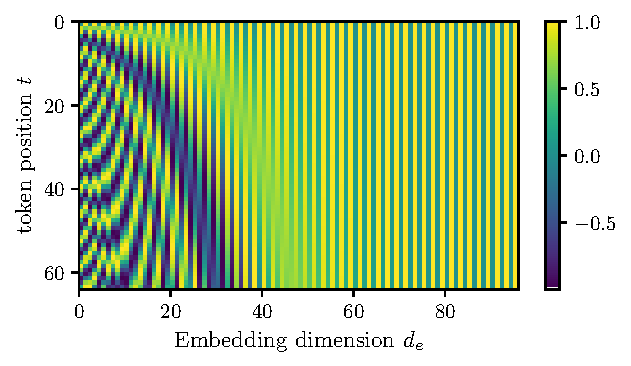
\includegraphics{positional-encoding.pdf}
    \caption[Positional Encoding of Transformer]{Positional encoding. The encoding is added onto the \gls{token} embeddings to add positional information. The heatmap visualizes the uniquely identifying pattern created from sine and cosine signals at increasing frequencies across the embedding dimension. Own work.}
    \label{fig:positional-embedding}
\end{figure}

The positional encoding is visualized in \cref{fig:positional-embedding}. One can see the alternating pattern between even and odd columns and the unique pattern for each \gls{token}'s position.

Using trigonometric functions for the positional embedding is favourable, due to being zero-centred and resulting in values in the closed range of $[-1,1]$. These properties are long known to promote convergence of neural networks \autocites[][8-9]{lecunEfficientBackProp2012}[][2]{ioffeBatchNormalizationAccelerating2015}.

The reason for encoding with both the sine and cosine is more subtle, as either one would suffice for absolute embeddings. \textcite[][6]{vaswaniAttentionAllYou2017} hypothesize, that besides learning the \emph{absolute} position i.e., fifth place in sequence, providing both sine and cosine also enables the model to attend to \emph{relative} positions, i.e., two places from a given \gls{token}.

The positional embedding is finally added per element to the token embedding to form a \gls{token}'s initial embedding $\gls{e}$. For the $\gls{t}$-th \gls{token} of a sequence $\gls{x}$, the embedding becomes:
\begin{equation}
    \gls{e}=\gls{W-e}\left[:, x[t]\right]+\gls{W-p}\left[:, t\right].
    \label{eq:positional-embedding}
\end{equation}

Intuitionally, adding the positional encoding leads to a rotation of the \gls{token} embedding in the embedding space. As the positional embedding is different for every location within the sequence, otherwise identical \glspl{token}, now have a distinct embedding.

\subsubsection{Attention}\label{sec:attention}

Recall from our discussion on token embeddings, that embeddings are not yet context-sensitive. The Transformer relies on an \emph{attention mechanism} to let tokens gather information from other tokens within the sequence and thereby encode the context onto the embeddings.

\textbf{Underlying Concept}

Attention can be thought of as a mapping between a query and a set of key-value pairs to an output. In general, the current token is first projected onto a query vector, and all tokens in the context are mapped to key and value vectors. Similar to a soft dictionary lookup, the goal is to retrieve the values from tokens in the context for which the keys are similar to the query and return an aggregate estimate of the values weighted by the similarity of the keys and the query. Naturally, if a token in the context is important for predicting the queried token, indicated by a high similarity, the value of the context token has a large contribution to the output \autocites[][5]{phuongFormalAlgorithmsTransformers2022}[][3]{vaswaniAttentionAllYou2017}.

Attention first appeared in \textcite[][4]{bahdanauNeuralMachineTranslation2016} and was popularized by \textcite[][4]{vaswaniAttentionAllYou2017}. The latter introduced a specific attention mechanism, known as \emph{scaled dot-product attention}, which we introduce in detail.

\textbf{Scaled Dot-Product Attention}

Analogous to before, \emph{scaled dot-product attention} estimates the similarity between queries and keys, as the dot product. The resulting attention scores are divided by some constant and normalized using a softmax function to obtain the attention weights. Multiplication of the attention weights with the values yields the outputs. Scaled dot-product attention is visualized in \cref{fig:transformer-architecture-overview} (left).

For computational efficiency, attention is performed simultaneously over multiple queries. Thus, the author's group queries, keys, and values in matrices. In matrix notation outputs are estimated as:

\begin{equation}
    \begin{aligned}
        \operatorname{Attention}(\mathbf{X},\mathbf{Z}) & = \mathbf{V} \operatorname{softmax}\left(\mathbf{S} / \sqrt{d_{\mathrm{attn}}}\right) \\
        \mathbf{S}                                      & = \mathbf{K}^{\top} \mathbf{Q}
    \end{aligned}
    \label{eq:attention}
\end{equation}
where $\mathbf{X} \in \mathbb{R}^{d_X\times \ell_X}$ and $\mathbf{Z} \in \mathbb{R}^{d_Z\times \ell_Z}$  are vector representations of the primary input sequence and of the context sequence. Both the primary and the context sequences are identical for the encoder but are different for the decoder. The query, key, and value matrices $\mathbf{Q}=\mathbf{W}_q \mathbf{X} + \mathbf{b}_q\mathbf{1}^{\top}$, $\mathbf{K}=\mathbf{W}_k \mathbf{Z} + \mathbf{b}_k\mathbf{1}^{\top}$, and $\mathbf{V}=\mathbf{W}_v \mathbf{Z} + \mathbf{b}_v\mathbf{1}^{\top}$ are linear projections of the input and context sequences, and $\mathbf{W}_q, \mathbf{W}_k \in \mathbb{R}^{d_{\mathrm{attn}\times d_{X}}}$; $\mathbf{W}_v \in \mathbb{R}^{d_{\mathrm{out}\times d_{Z}}}$; $\mathbf{b}_q, \mathbf{b}_k \in \mathbb{R}^{d_{\mathrm{attn}}}$, and $\mathbf{b}_v \in \mathbb{R}^{d_{\mathrm{out}}}$ are learnable parameters. The dimensionality of the attention mechanism, $d_{\mathrm{attn}}$, is typically a fraction of the model dimensionality to accelerate computation. Likewise, the output dimension, $d_{out}$, is another hyperparameter to the models. The attention scores are $\mathbf{S}$, which are scaled by $\sqrt{d_{\mathrm{attn}}}$ to avoid unstable gradients, and the softmax activation normalizes all scores. As normalized attention scores have a clear interpretation as the weights how much a token contributes to the model's output, the attention mechanism provides a window into the model, which we explore in \cref{sec:feature-importance-measure}.

\textbf{Multi-Head Attention}

Rather than relying on a single attention function, \textcite[][4--5]{vaswaniAttentionAllYou2017} introduce multiple \emph{attention heads}, which perform attention in parallel on $H$ \emph{different} linear projections of queries, keys, and values. The \emph{multi-head attention} enables the model to learn richer representations of the input, as attention heads operate independently, they can pick up unique patterns or focus on different positions in the sequence at once. Multi-head attention is visualized in \cref{fig:transformer-architecture-overview} (centre).

Exemplary for machine translation, \textcite[][5795]{voitaAnalyzingMultiHeadSelfAttention2019} show, that heads serve indeed distinct purposes like learning positional or syntactic relations between tokens. It is conceivable, that for tabular data this maps to dependencies between features. In practice, Transformers may not leverage all attention heads and some heads could even be pruned without impacting the performance \autocites[][9]{michelAreSixteenHeads2019}[][5805]{voitaAnalyzingMultiHeadSelfAttention2019}.

Multi-head attention can be computed as:

\begin{equation}
    \begin{aligned}
        \operatorname{MHAttention}(\mathbf{X}, \mathbf{Z}) & = \mathbf{W}_{o}\left[\mathbf{Y}^{1};\mathbf{Y}^{2};\ldots;\mathbf{Y}^{H} \right] + \mathbf{b}_{o}\mathbf{1}^{\top} \\
        \mathbf{Y}^{h}                                     & = \operatorname{Attention}(\mathbf{Q}^h, \mathbf{K}^h, \mathbf{V}^h)
    \end{aligned}
\end{equation}
The query, key, and value matrices  $\mathbf{Q}^{h}=\mathbf{W}^h_q \mathbf{X} + \mathbf{b}^h_q\mathbf{1}^{\top}$, $\mathbf{K}^{h}=\mathbf{W}_k^h \mathbf{Z} + \mathbf{b}_k^h\mathbf{1}^{\top}$, and $\mathbf{V}^{h}=\mathbf{W}_v^h \mathbf{Z} + \mathbf{b}_v^h\mathbf{1}^{\top}$ are obtained from linear projections of the input and context sequences unique per head. Again, $\mathbf{W}^{h}_{q} \in \mathbb{R}^{d_{\mathrm{attn}}\times d_{X}}$; $\mathbf{W}^{h}_{k}, \mathbf{W}^{h}_{v} \in \mathbb{R}^{d_{\mathrm{attn}}\times d_Z}$; $\mathbf{b}^h_q, \mathbf{b}^h_k \in \mathbb{R}^{d_{\mathrm{attn}}}$, and $\mathbf{b}^h_v \in \mathbb{R}^{d_{\mathrm{mid}}}$ are used for projection. Typically, the dimensionality of the attention heads, $d_{\mathrm{mid}}$, is reduced to $d_{\mathrm{attn}}/H$ to match the computational cost of single-head attention. The output dimensionality $d_{\mathrm{out}}$ is restored with a final linear projection through the weight matrix $\mathbf{W}_{o} \in \mathbb{R}^{d_{\mathrm{out}}\times Hd_{\mathrm{mid}}}$ and bias $\mathbf{b}_o \in \mathbb{R}^{d_{\mathrm{out}}}$ applied to the concatenated results of the attention heads.

The concatenated and projected output of the attention heads is then passed to the point-wise feed-forward networks, which enables interaction between the head's outputs. We discuss position-wise feed-forward networks in \cref{sec:position-wise-ffn}.

\textbf{Masked Self-Attention and Cross-Attention}


In the \cref{eq:attention}, tokens can attend to any preceding or subsequent token without restrictions. Thus, the full \emph{bidirectional context} is used. This design is optimal for the encoder, where the entire input sequence shall serve as the context.

For the decoder, the self-attention is modified to \emph{masked self-attention} and \emph{cross-attention} mechanism. First, causal masking is required to achieve autoregressive sequence generation in the decoder. The context is \emph{unidirectional}, where a token is only allowed to attend to itself or all previously generated tokens. Second, the decoder uses \emph{cross-attention} to connect between the encoder and decoder. Other than in the self-attention mechanism, where keys, values and queries are generated from the same sequence, keys and values come from the encoder and queries are provided by the decoder. As our focus is on encoder-only architectures, we refer the reader to \textcite[][16--17]{raffelExploringLimitsTransfer2020} for an in-depth treatment of both topics.

\subsubsection{Position-wise Feed-Forward Networks}\label{sec:position-wise-ffn}

The attention mechanism enables \glspl{token} to attend to other inputs in the immediate context. To retain general information on the task, outside and independent of the immediate context, each Transformer block adds a point-wise \gls{feed-forward-network}, which acts as a persistent memory to the model \autocite[][3]{sukhbaatarAugmentingSelfattentionPersistent2019}.

The network consists of a linear transformation, followed by a non-linear activation function and a second linear layer. For the $l$-th layer, the \gls{MLP} is given by
\begin{equation}
    \gls{X} = \gls{X}+\mathbf{W}_{\mathrm{mlp} 2}^l \operatorname{ReLU}\left(\mathbf{W}_{\mathrm{mlp} 1}^l \gls{X}+\mathbf{b}_{\mathrm{mlp} 1}^l 1^{\top}\right)+\mathbf{b}_{\mathrm{mlp} 2}^l 1^{\top},
\end{equation}

with $\mathbf{W}_{\mathrm{mlp } 1}^l \in \mathbb{R}^{d_{\mathrm{mlp}} \times d_{e}}, \mathbf{b}_{\mathrm{mlp} 1}^l \in \mathbb{R}^{d_{\mathrm{mlp}}}, \mathbf{W}_{\mathrm{mlp} 2}^l \in \mathbb{R}^{d_{e}} \times d_{\mathrm{mlp}}$ and $\mathbf{b}_{\mathrm{mlp} 2}^l \in \mathbb{R}^{d_{e}}$ being learnable parameters identical for all \glspl{embedding} in the layer. The network is applied to each embedding separately and identically.

\textcite[][9]{vaswaniAttentionAllYou2017} set the hidden dimension to be two to eight magnitudes of the embedding dimension. The large capacity strengthens the model's ability to retain information but also contributes significantly to the high computational requirements and memory footprint of Transformers \autocites[][5]{tayEfficientTransformersSurvey2022}[][1]{kitaevReformerEfficientTransformer2020}. Both linear transformations are separated by a \gls{ReLU} \gls{activation-function} \autocite[][318]{glorotDeepSparseRectifier2011} to introduce non-linearities to the network.

Like the attention layer, the position-wise \gls{FFN} is surrounded by residual connections, followed by layer normalization (cp. \cref{sec:residual-connections-layer-norm}). Both are vital for the training process and convergence of the overall network. Optionally, dropout \autocite[][1930]{srivastavaDropoutSimpleWay} is added to prevent the model from \gls{overfitting}.

\subsubsection{Residual Connections and Layer Normalization}\label{sec:residual-connections-layer-norm}

% Recall from earlier chapters, that the encoder stacks multiple Transformer blocks, each of which consists of several sublayers, resulting in a deep network. While depth is inevitable to learn hierarchical representations, the training of such a network is complicated. As neural networks are commonly trained using backpropagation, which relies on the gradient of the error to be propagated through the network starting at the last layer, \glslink{exploding-gradient}{vanishing or exploding gradients} pose a major difficulty in training deep neural nets \autocite[][1]{heDeepResidualLearning2015}. Without countermeasures, stacking multiple layers in the encoder and decoder of the Transformers impedes the gradient information to flow efficiently through the network and hampers the training behaviour \autocite[][1811]{wangLearningDeepTransformer2019}.

As a remedy, \textcite[][3]{vaswaniAttentionAllYou2017} employ residual connections around each sublayer, whereby the output of the sublayer is added element-wisely to its input. Intuitively, the residual connection provides an alternative path for information to flow through the network, since some information can bypass the sublayer and thereby reach deeper layers within the stack. Vanishing or \glspl{exploding-gradient} are also mitigated, as gradients can bypass the sublayer, eventually contributing towards an easier optimisation \autocite[][3591]{liuRethinkingSkipConnection2020}. Residual connections moreover help to preserve the positional embeddings (cp. \cref{sec:positional-encoding}), as the layer's inputs are maintained in the identity mapping. Another technique to improve the training behaviour is layer normalization.

\textcite[][3]{vaswaniAttentionAllYou2017} extensively draw on layer normalization \autocite[][4]{baLayerNormalization2016} after the multi-head attention and feed-forward sublayers. It is used for normalizing the activations of the sublayer and to stabilize and accelerate the training of the network \autocite[][2]{baLayerNormalization2016}. The normalization statistics are calculated separately for every instance, which guarantees scalability across different batch sizes.

Until now it remains unclear, how the layer normalization intertwines with the sublayers and the residual connections. Transformers are distinguished by the order in which layer normalization is added into the pre-norm and post-norm Transformer. Post-norm Transformers add layer normalization to the sublayer \emph{after} adding the input from the residual connections. The arrangement is depicted in \cref{fig:transformer-architecture-overview}. In contrast for pre-norm Transformers, the normalization is applied \emph{before} the self-attention and feed-forward sublayers and inside the residual connections. Pre-norm requires one additional normalization layer to pass only well-conditioned outputs from the Transformer block to the successive layers \autocite[][5]{xiongLayerNormalizationTransformer2020}.

% \textcite[][3]{vaswaniAttentionAllYou2017} employ post-layer normalization, but recent research has shown a shift towards pre-norm setups \autocite[][4]{narangTransformerModificationsTransfer2021}. Parts of the widespread adaption lie in faster training and omitting of the need for costly learning rate warm-up stages, whereby the learning rate is initially decreased to keep the gradients balanced \autocites[][2]{xiongLayerNormalizationTransformer2020}[][8]{liuUnderstandingDifficultyTraining2020}. In addition, post-norm Transformers have been found brittle to train and prone to convergence failures with its root cause in \glslink{exploding-gradient}{vanishing gradients}, \glspl{exploding-gradient}, and an overall higher dependency on the residual stream \autocites[][8]{liuUnderstandingDifficultyTraining2020}[][1812]{wangLearningDeepTransformer2019}. Pre-norm Transformers, although they may sacrifice some performance, introduce a certain robustness to the training process. We come back to this property in our discussion on the FT-Transformer.

\subsubsection{FT-Transformer}\label{sec:fttransformer}

Many of the previous concepts can be adapted to the tabular domain with minor architectural changes. We cover FT-Transformer as a state-of-the-art adaption.

\begin{figure}[ht]
    \centering
    {\renewcommand\normalsize{\scriptsize}
        \normalsize
        \input{./Graphs/fttransformer.pdf_tex}}
    \caption[Overview Over the FT-Transformer Architecture]{Overview Over the Architecture of FT-Transformer. The FT-Transformer uses a pre-norm arrangement and operates on numerical and categorical embeddings. Own work inspired by \textcite[][4--5]{gorishniyRevisitingDeepLearning2021}.}
    \label{fig:fttransformer}
\end{figure}

\textcite[][5]{gorishniyRevisitingDeepLearning2021} propose with FT-Transformer an adaption, that pairs an embedding unit for both numerical and categorical inputs, dubbed the feature tokenizer, with a Transformer. The complete architecture is depicted in \cref{fig:fttransformer}. Notably, the Transformer units use a pre-norm setup for easier optimisation, whereby the very first normalization layer in the encoder is removed due to a propitious performance \textcite[][17]{gorishniyRevisitingDeepLearning2021}. The upstream feature tokenizer transforms every feature in $\mathbf{x}$ to their embeddings. The embeddings are given by \cref{eq:numerical-embeddings,eq:categorical-embeddings}.

Recall from our discussion on self-attention (cp. \cref{sec:attention}), that each \gls{token} encodes the \glspl{token} within the sequence. Based on this notion, \textcite[][4174]{devlinBERTPretrainingDeep2019} prepend a specialised $\mathtt{[CLS]}$ \gls{token} to the sequence, which stores the sequence's aggregate representation. Like any other \gls{token}, the $\mathtt{[CLS]}$ \gls{token} is embedded first and contextualised in the encoder. Its final hidden state is then used for classification.

\textcite[][4]{gorishniyRevisitingDeepLearning2021} adapt the idea of a $\mathtt{[CLS]}$ \gls{token} for tabular representation models. Similar to the embeddings of categorical or numerical features, the embedding of the $[\mathtt{CLS}]$ \gls{token} $\gls{e}_\mathtt{[CLS]} \in \mathbb{R}^{d_{e}}$ is prepended to the column embeddings with $\gls{X} = \left[\gls{e}_\mathtt{[CLS]}, \gls{e}_1, \ldots \gls{e}_{M}\right]$, where $\gls{X} \in \mathbb{R}^{d_{e} \times M +1}$. Like before, $\gls{X}$ is passed through a stack of Transformer layers. The updated representation of the $\mathtt{[CLS]}$ \gls{token} is used exclusively for prediction:
\begin{equation}
    P=\mathtt{linear}\left(\mathtt{ReLU}\left(\mathtt{layer\_norm}\left(\gls{X}\left[:,0\right]\right)\right)\right).
    \label{eq:bert-ft}
\end{equation}
% TODO: Add softmax, think about ReLU

\textcite[][8]{gorishniyRevisitingDeepLearning2021} achieve state-of-the-art performance through numerical and categorical embeddings. Embedding both categorical and numerical inputs enables the Transformer to attend to all other features, but at an considerable computational cost, that may only be justified by higher classification accuracies.

In the subsequent section, extend all previous models including FT-Transformer for learning on partially labelled data.

\newpage
\section{Semi-Supervised Approaches}\label{sec:semi-supervised-approaches}
\subsection{Framing as a Semi-Supervised Learning Problem}\label{sec:problem-framing-2}

The supervised approaches depend on the availability of the trade initiator as the true label. Yet, obtaining the label is often restricted to the rare cases, where the trade initiator is provided by the exchange or to subsets of trades where the initiator can be inferred through matching procedures (cp. \cref{sec:trade-initiator}), which may bias the selection. Unlabelled trades, though, are abundant and can help improve the generalisation performance of the classifier. This concern is adressed by semi-supervised methods.

Semi-supervised methods leverage partially-labelled data by learning an algorithm on unlabelled instances alongside with true labels \autocite[][6]{chapelleSemisupervisedLearning2006}. They are centred around the semi-supervised assumption of smoothness, which states that if two samples, say $\mathbf{x}_{1}$ and $\mathbf{x}_{2}$, are nearby in a high-density region, their class labels $y_{1}$ and $y_{2}$ should also be similar. Vice versa, if data points are separated by a low-density region, their labels may be different \autocite[][5]{chapelleSemisupervisedLearning2006}.

\begin{figure}[h]
    \centering
    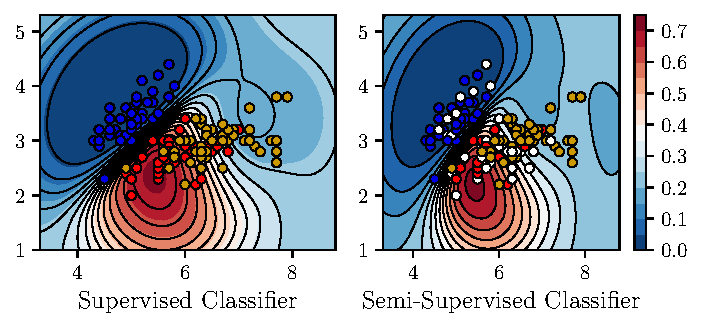
\includegraphics[width=0.8\linewidth]{decision-boundary-semi-supervised.pdf}
    \caption[Decision Boundary of a Supervised and Semi-Supervised Classifier]{Decision Boundary of a Supervised and Semi-Supervised Classifier. Own work.}
    \label{fig:supervised-semi-supervised}
\end{figure}

Applied to trade classification, with semi-supervised methods we implicitly assume that trades with similar features, such as a common trade price and quotes, conform to the same class. The purpose of unlabelled trades is to help efficiently determine the boundary around regions of neighbouring trades resulting in an improved generalisation performance. A visualization of a decision boundary of (semi-)supervised classifier is given in \cref{fig:supervised-semi-supervised}.

The semi-supervised setting requires extending our notation from \cref{sec:problem-framing}, by distinguishing between labelled and unlabelled instances. Like before, $\mathcal{S}=\left\{\left(\mathbf{x}_i, y_i\right)\right\}_{i=1}^N$ denotes all labelled trades. Unlabelled datapoints are stored in separate set $\mathcal{U} = \left\{\mathbf{x}_i\right\}_{i=1}^{K}$. Our coverage of semi-supervised approaches includes self-training for gradient boosting and pre-training of Transformers, which we derive from a subsequent discussion.

\subsection{Selection of Approaches}\label{sec:selection-of-approaches-1}

Our goal is to extend gradient-boosted trees and Transformers for the semi-supervised setting to make use of the abundant, unlabelled trade data. We are aimed to make minimally intrusive changes to maintain a fair comparison with the supervised counterparts.

\textbf{Gradient Boosting}

The success of supervised gradient boosting led to the development of gradient boosting for the semi-supervised setting. An early work of \textcite[][3--4]{dalche-bucSemisupervisedMarginBoost2001} explores replacing supervised weak learners, i.e., regression trees, with semi-supervised weak learners, i.e., mixture models and minimises a loss function over labelled and unlabelled instances. Another line of research, including \textcites[][290--291]{bennettExploitingUnlabeledData2002}[][2003--2004]{mallapragadaSemiBoostBoostingSemiSupervised2009}, retain supervised weak learners to generate pseudo labels of unlabelled instances per iteration. True labelled and pseudo-labelled data is then used in fitting weak learners of subsequent iterations. Approaches differ regarding the selection criterion of the pseudo-labelled instances. Both lines of work, however, require changes to the boosting procedure or the base learners.

An alternative is to pair gradient boosting with self-training. Self-training is a wrapper algorithm around a supervised classifier, that incorporates its most-confident predictions of unlabelled instances into the training procedure \autocite[][190]{yarowskyUnsupervisedWordSense1995}. Other than before, pseudo labels are generated only from the fully-fledged ensemble and the ensemble is grown multiple times. Being a model-agnostic wrapper, the self-training classifier does not change the base classifier and ensures maximum comparability.  Its widespread adoption in literature reinforces its appeal as a compelling solution for semi-supervised trade classification.

\textbf{Transformer}

Whilst Transformers could be combined with self-training, a more promising approach is to pre-train Transformers on unlabelled data, and then fine-tune the network on the remaining labelled instances. Various studies report unanimously performance improvements from pre-training tabular Transformers, including \textcites[][8]{somepalliSaintImprovedNeural2021}[][7]{huangTabTransformerTabularData2020}.

Until now we assumed the parameters e.g., weights and biases, of the Transformer to be initialized randomly. The joint goal of pre-training objectives is to initialize a neural network with weights that capture expressive representations of the input and thereby improve generalization performance over a random initialization when fine-tuning on a specific task \autocite[][12]{erhanWhyDoesUnsupervised}. Pre-training objectives for tabular data differ vastly in their methodology and are often directly adapted from other domains including \gls{MLM}, \gls{RTD}, or contrastive learning. As such, \textcite[][7]{huangTabTransformerTabularData2020} adapt \gls{MLM}, whereby features are randomly masked and the objective is to reconstruct the original input. Pre-training by \gls{RTD} aims to identify randomly replaced features and recover a binary mask used for replacement \autocite[][7]{huangTabTransformerTabularData2020}. \textcites[][3]{bahriSCARFSelfsupervisedContrastive2022}[][4--5]{yoonVIMEExtendingSuccess2020} reconstruct both the binary feature mask and the original input simultaneously. \textcite[][3]{somepalliSaintImprovedNeural2021} alter the methodology of \textcite[][4--5]{yoonVIMEExtendingSuccess2020} through a contrastive loss function.

With a multitude of methods, tested on different datasets and neural architectures, a fair comparison between pre-training methods is tedious. Yet, \textcite[][2-3]{rubachevRevisitingPretrainingObjectives2022} provide guidance in selecting objectives. Among the pre-training objectives that they benchmark, a tabular adaptation of the \gls{MLM} objective \autocite[][4174]{devlinBERTPretrainingDeep2019} was among the best-performing approaches. The \gls{MLM} objective is easy to optimise, unsupervised, and leaves the model architecture unaltered, which makes \gls{MLM} a compelling choice for pre-training on unlabelled data.

The next chapter covers self-training in detail.

%TODO: Caruana caruanaObtainingCalibratedProbabilities -> ok for trees, but we do not optimize probabilities but the logits!
\subsection{Gradient Boosted Trees With Self-Training}\label{sec:extensions-to-gradient-boosted-trees}

Self-training is a wrapper algorithm around a probabilistic classifier, that incorporates its predictions of unlabelled instances as pseudo labels \autocite[][190]{yarowskyUnsupervisedWordSense1995}.

Initially, a base classifier is fitted on the labelled data points in a supervised manner. The classifier then assigns labels, so-called pseudo labels, to unlabelled instances. A subset of unlabelled instances with high-confidence predictions is selected, removed from the unlabelled dataset and added to labelled data dataset. A new classifier is then retrained on the labelled and pseudo-labelled instances \autocite[][190--192]{yarowskyUnsupervisedWordSense1995}. The process is repeated for several iterations until an abortion criterion applies, such as the maximum number of iterations is exhausted or when no unlabelled instances are left to label.

Recall from our discussion on gradient-boosted trees in \cref{sec:gradient-boosting-procedure} that we optimised for the cross-entropy loss on the training set. When coupled with self-training in each training iteration the classifier $F$ now jointly minimises the loss over the labelled samples $\mathcal{S}$ and the pseudo-labelled samples $\not{\mathcal{U}}$:
\begin{equation}
    L_{\mathrm{ST}}=\frac{1}{\left|\mathcal{S}\right|} \sum_{(\mathbf{x}, y) \in \mathcal{S}} L(F(\mathbf{x}), y)+\frac{\epsilon}{\left|\not{\mathcal{U}}\right|} \sum_{(\mathbf{x}, \tilde{y}) \in \not{\mathcal{U}}} L(F(\mathbf{x}), \tilde{y})+\lambda\|F\|^2,
\end{equation}
where $\epsilon$ is a hyperparameter to control the impact of the pseudo-labelled data, $\tilde{y}$ is the pseudo-labelled instance, and $\lambda$ weights the regularisation term \autocite[][4]{aminiSelfTrainingSurvey2023}.

In every iteration, only unlabelled instances are added to the training set, for which the predicted class probability exceeds a confidence threshold, say $\tau$. This approach has implications, as highlighted by \textcite[][2]{chenDebiasedSelfTrainingSemiSupervised2022}. The threshold $\tau$ becomes an important hyperparameter in controlling that no noisy labels are added to the training set, but a restriction to highly-confidence samples may lead to a data bias and over-confidence in the prediction. Self-training is prone to a confirmation bias, as confident but wrong pseudo labels are erroneously incorporated into the training set, which in effect leads to a propagation of errors in the subsequent training rounds.

At the same time, self-training puts a high emphasis on the correctness of the probability estimates in the base classifier. This is problematic for decision trees, known to produce poor probability estimates, as probabilities are derived from the class frequency in the leaf node containing few samples \autocite[][357--358]{tanhaSemisupervisedSelftrainingDecision2017}. However, as gradient boosting, directly optimises for the cross-entropy loss, the problem found for its ensemble member no longer occurs.

Independent of the base classifier, self-training increases computational cost, as training is repeated over several iterations on a growing training set \autocite[][9]{zophRethinkingPretrainingSelftraining2020}.

Despite these limitations, the potentially improved decision boundary outweighs the concerns.

\subsection{Transformers with Pre-Training}\label{sec:extensions-to-transformer}

\gls{MLM} is a pre-training task proposed for the use in language models by  \textcite[][4174]{devlinBERTPretrainingDeep2019}. The core idea of \gls{MLM} is to randomly mask \SI{15}{\percent} of the tokens, i.e., words, in the input sequence. Eventually, the model learns to predict the original token of the now masked token through the tokens in the bidirectional context. Separately for each token, the final hidden state of the masked token is fed through an softmax activation to obtain the predicted probability distribution for the original token and the cross entropy loss is used to compare against the true distribution. For masking, the authors introduce an additional $\mathtt{[MASK]}$ token, that extends the vocabulary \autocite[][4174]{devlinBERTPretrainingDeep2019}. 

A caveat of \gls{MLM} is, that the mask token only appears during pre-training, but not in fine-tuning, causing a mismatch between the pre-training and fine-tuning task. The issues is mitigated by a sophisticated replacement strategy of the masked token: only \SI{80}{\percent} of the time the token is replaced with the $\mathtt{[MASK]}$ token, in \SI{10}{\percent} it remains unchanged, and replaced with a random token \autocite[][4174]{devlinBERTPretrainingDeep2019}. The random or no replacement avidly avoids overfitting.

Applied to tabular datasets, \gls{MLM} transfers to randomly masking features or elements in $\mathbf{x}_{i}$ instead of sequences.  Previous adaptions for tabular data, e.g., \textcites[][3]{huangTabTransformerTabularData2020}[][8]{levinTransferLearningDeep2022}, simplify the replacement strategy to substitution with the $\mathtt{[MASK]}$ token only, and try to reconstruct the original features.  Other than in the language case, reconstruction of masked features requires distinct classification heads per feature and adequate loss functions, which significantly increases the memory footprint and computational demand \autocite[][16]{levinTransferLearningDeep2022}.

% A lightweight alternative is presented in \textcite[][4]{rubachevRevisitingPretrainingObjectives2022}. Here, features are masked and replaced. The objective is now to predict the binary mask $\mathbf{m}_{i}\in \{0,1\}^{M}$ vector corresponding to $\mathbf{x}_{i}$, indicating which features, or entries in $\mathbf{x}_{i}$, have been corrupted.

In summary, \gls{MLM} can help to learn expressive representations of the input, even if the true label is unavailable. Given previous research, we expect pre-training to improve the performance of the FT-Transformer and match or exceed the one of the \gls{GBM}.

\newpage
\addtocontents{toc}{\protect\newpage}
\section{Empirical Study (19.5~p)}\label{sec:empirical-study}

In this Section, we demonstrate the effectiveness of gradient boosting and Transformers for trade classification. We benchmark against the \gls{LR}, \gls{EMO}, and \gls{CLNV} algorithm, as well as hybrids involving the trade size rule and depth rule on two datasets of option trades recorded at the \gls{ISE} and \gls{CBOE}.

Experiments were conducted on shared nodes of the bwHPC cluster, with 10 assigned Intel Xeon Gold 6230 cores at \SI{2.1}{\GHz}, an NVIDIA V100 \SI{32}{\giga\byte}, and \SI{92.160}{\giga\byte} random access memory running Red Hat Enterprise Linux release 8.4. For reproducibility, the implementation and experiment tracking are publicly available~\footnote{Code is available at~\url{https://github.com/KarelZe/thesis}. Experiments are tracked at \url{https://wandb.ai/fbv/thesis}.}.

The subsequent section provides details on the datasets.

\subsection{Data and Data Preparation (6 p)}\label{sec:data-and-data-preparation}

The following chapter describes the construction of datasets, that suffice the data requirements of classical trade classification rules and for our machine learning models. We also discuss how we define and infer the trade initiator.
The following chapter describes the construction of datasets, that suffice the data requirements of classical trade classification rules and for our machine learning models. We also discuss how we define and infer the trade initiator.

\subsubsection{Data Collection}\label{sec:data-collection}

\textbf{Data Sources}

Testing the empirical accuracy of our approaches requires option trades where the true initiator is known. To arrive at labelled sample, we combine data from four individual data sources. Our primary source is LiveVol, which records option trades executed at US option exchanges at a transaction level. We limit our focus to option trades executed at the \gls{CBOE} and \gls{ISE}. LiveVol contains both trade and matching quote data. Like most proprietary data sources, it does not distinguish the initiator nor does it include the involved trader types. For the \gls{CBOE} and \gls{ISE} exchange, the \gls{ISE} Open/Close Trade Profile and \gls{CBOE} Open-Close Volume Summary contain the buy and sell volumes for the option series by trader type aggregated on a daily level. A combination of the LiveVol dataset with the open/close data, allows us to infer the trade initiator for a subset of trades. For evaluation and use in some of our machine learning models, we acquire additional underlying and option characteristics from IvyDB's OptionMetrics.

\textbf{Trade Initiator}

In \cref{sec:trade-initiator} we discussed three views on the trade initiator. As our data sources do not provide the order entry times or order types for both sides of the trade, we define the trade initiator based on the position relative to the market maker, who caters to the liquidity demand. More specifically, we classify customer trades as buyer-initiated if the trade is due to a customer buy order and as seller-initiated for customer sales. As previous literature, e.g., \textcite[][4276]{garleanuDemandBasedOptionPricing2009} suggests that trader types, for example, proprietary traders, have a similar role to market makers by supplying liquidity, we limit our analysis to trades between customers and market makers for which the picture is unambiguous. Our definition is consistent with the in \textcite[][8]{grauerOptionTradeClassification2022}.

\textbf{Sample Construction}

Our sample construction follows \textcite[][7--9]{grauerOptionTradeClassification2022}, fostering comparability between both works. We acquire transaction-level options trade data for all major US exchanges from LiveVol. The dataset is tabular, and each record is time-stamped to the second. For each transaction, the executing exchange, trade price, trade volume, quotes and quote sizes for the exchanges where the option is quoted, as well as the \gls{NBBO} are recorded. This is sufficient to estimate the quote rule, depth rule, and trade size rule. In addition, for tick-based algorithms, we add the previous and subsequent distinguishable trade prices. We can uniquely identify the traded option series from a distinct key consisting of the underlying, expiration date, option type and strike price. Our analysis is conducted on transactions at the \gls{ISE} and \gls{CBOE}. To purge the data of potential errors, we filter out option trades with a trade price equal to or less than zero and eliminate trades with a negative or zero trade volume as well as large trades with a trading volume exceeding \num{10000000} contracts. We further remove cancelled or duplicated trades and eliminate entries with multiple underlying symbols for the same root.

The open/close datasets for the \gls{ISE} and \gls{CBOE} contain the daily buy and sell volumes for the option series by trader type, the trade volume and whether a position was closed or opened. Four trader types are available: customer, professional customer, broker/dealer, and firm proprietary. Customer orders are placed by a retail trader or a member of the exchange on behalf of the customer. Professional customers are distinguished from the former by a high trading activity ($\geq390$ orders per day over one month period). Likewise, trades by a member are classified as proprietary, if executed for their account or broker/dealer if placed for non-members of the exchange \autocite[][2]{nasdaqincFrequentlyAskedQuestions2017}. Trades of customers and professional customers are detailed by trade volume ($\leq 100$; 101--199; $> 199$ contracts). As well as, if a position is newly opened or closed. We first sum buy and sell orders of all trader types and volumes to obtain the daily trading volumes at the \gls{ISE} or \gls{CBOE} per option series and day. Similarly, we calculate the aggregate of the customer buy and sell volumes identified by the account type customer. Despite commonalities, we do not consider professional customers as customers, as the trader type became only available mid-sample.
% TODO:Why don't we include professional customers? 

To infer the true label, we exploit that, if there were only customer buy or sell orders, hence the customer buy or sell volume equals the daily trading volume, we can confidently sign all transactions for the option series at the specific date and exchange as either buyer- or seller-initiated. The applicability of our labelling approach is constrained by the existence of non-customer or simultaneous customer buy and sell trades. The so-obtained trade initiator is merged with the LiveVol trades of the exchange based on the unique key for the option series.

For the \gls{ISE} trades, our matched sample spans from 2 May 2005 to 31 May 2017 and includes \num{49203747} trades. The period covers the full history of \gls{ISE} open/close data up to the last date the dataset was available to us. Our matched \gls{CBOE} sample consists of \num{37155412} trades between 1 January 2011 and 31 October 2017. The sample period is governed by a paradigm shift in the construction of the \gls{CBOE} open/close dataset and the most recent trade in our LiveVol subscription.

Following our initial rationale for using semi-supervised methods, we reserve unlabelled trades between 24 October 2012 and 24 October 2013 at the \gls{ISE} for pre- and self-training. We provide further details in \cref{sec:train-test-split}. Since Livevol doesn't distinguish by trader types, this dataset includes both customer and non-customer trades.

While our procedure makes the inference of the true trade initiator partly feasible, concerns regarding a selection bias due to the excessive filtering have to be raised. We address these concerns as part of our exploratory data analysis in \cref{sec:exploratory-data-analysis}, in which we compare unmerged and merged sub-samples.

\subsubsection{Exploratory Data Analysis (2~p)}
\label{sec:exploratory-data-analysis}

In the following chapter, we motivate feature engineering, present our feature sets and discuss strategies for transforming features into a form that accelerates and advances the training of our models.
\subsubsection{Data Preprocessing}\label{sec:data-preprocessing}

Classical algorithms infer the initiator of the trade from the \emph{raw} price and quote data. We employ feature engineering to pre-process input data and enhance the convergence and performance of our machine-learning models. Gradient-boosted trees and neural networks, though flexible estimators have limitations in synthesizing new features from existing ones, as demonstrated in empirical work on synthetic data by \textcite[][5--6]{heatonEmpiricalAnalysisFeature2016}. Specifically, ratios, standard deviations, and differences can be difficult for these models to learn and must therefore be engineered beforehand.

\textbf{Feature Sets}

To establish a common ground, we derive three sets of features from raw data. The feature sets are motivated by features inherent to classical trade classification rules and are consequently derived from quote and price data. Except for a third feature set, which includes additional option characteristics. Differentiated feature sets improve the transferability of our results.

All feature sets, their definition and origin are documented in \cref{app:feature-sets}. We aid the models by estimating the change in trade price between the previous and successive distinguishable trades. This is identical to the criterion used in the (reverse) tick rule, but in a non-quantized fashion to enforce a richer decision boundary and to surpass hard cut-off points. Similarly, the proximity of the trade price to the quotes, which is the decisive criterion in the quote rule and hybrids' there-off is added. The feature value ranges from $\left(-\infty,\infty\right)$ and is $-1$ for trades at the bid, 0 for trades at the mid, and 1 for trades at the ask. Quotes and trade prices are also incorporated as-is.

Our second feature set extends the first feature set by the trade size and size of the quotes, required to estimate hybrid rules involving the depth rule and trade size rule. Both rules are state-of-the-art when paired with hybrid algorithms and are thus both benchmark and source for features. We model the depth rule as the ratio between ask and bid sizes and the trade size rule as the ratio between the size of the trade and the quoted bid and ask sizes ranging between $\left[0,1\right]$. The trade price and midspread required for the depth rule are already encompassed in the first feature set.

Our largest feature set also incorporates option characteristics, including the strike price, the time to maturity, the moneyness, the option type and issue type as well as the underlying and traded volume of the option series. By providing the model with option-specific features, we hope to make nuances between the underlying, security types, and option types learnable.

Arguably, our models have simultaneous access to the previous and successive trade prices and quotes for both the exchange and the NBBO, which is an advantage over base rules. As we benchmark against various, stacked hybrid rules, the data requirements are comparable. We emphasize this aspect, as it is neglected in previous works \autocites[][485]{blazejewskiLocalNonParametricModel2005}[][48]{ronenMachineLearningTrade2022}[][9]{rosenthalModelingTradeDirection2012}.

\textbf{Numerical Features}

Pricing or quote data can often not be fully reconstructed, resulting in missing values across all features. Decision trees and ensembles thereof can inherently handle $\mathtt{[NaN]}$ values by discarding missing values in the splitting procedure \autocite[][150--152]{breimanClassificationRegressionTrees2017} or by incorporating missing values into the splitting criterion \autocite[][951]{twalaGoodMethodsCoping2008}. Transformers require missing values to be imputed beforehand, as a $\mathtt{[NaN]}$ value cannot be propagated through the network. We choose zero imputation for being a single-pass strategy that minimises data leakage and allows gradient-boosted trees and neural networks to separate imputed values from observed ones. With a low degree of missing values, the impact on the final result is minuscule.

Price and size-related features exhibit positive skewness, as brought up in \cref{sec:exploratory-data-analysis}. Tree-based learners are unaffected by the feature scale, as the splitting process is based on the purity of the split but not on the scale of splitting value (cp. \cref{sec:decision-tree}). To avoid the tails of the distribution dominating the weight updates of neural networks, we apply power transformations, which transform the distribution of features to be Gaussian-like. Apart from quantization effects, gradient-boosted trees are unaffected. We determine the power transformation using the Box-Cox procedure \autocite[][214]{boxAnalysisTransformations2022}, given by:

\begin{equation}
    \mathbf{X}^{*}\left[:,j\right]= \begin{cases}\frac{1}{\lambda}(\mathbf{X}\left[:,j\right]^\lambda-1), & \lambda \neq 0 \\ \log (\mathbf{X}\left[:,j\right]),& \lambda=0\end{cases}.
    \label{eq:box-cox-test}
\end{equation}

Here, $\lambda$ is the power parameter and determines the specific power function. It is estimated by optimising for the Gaussian likelihood on the training set. As shown in \cref{eq:box-cox-test}, a value of $\lambda=0$ corresponds to a log-transform, while $\lambda=1$ leaves the feature unaltered. As the test is only defined on positive $\mathbf{X}\left[:,j\right]$, we follow common practice by adding a constant if needed. Our estimates for $\lambda$ are documented in the \cref{app:power-transforms-of-features}. Based on the results of the Box-Cox test, we apply a common $\widehat{\mathbf{X}}\left[:,j\right]=\log(\mathbf{X}\left[:,j\right])$ transform on all price and size-related features with the effect of compressing large values and expanding smaller ones~\footnote{More specifically, $\mathtt{log1p}$ is used to improve numerical stability in floating point calculations. Results are not affected.}.

Note that, the use of the Box-Cox transform is different from its originated purpose. In feature engineering, the transformation is used in an unsupervised fashion, as the transformation's outcome is not directly used in the model. Also, the transform is applied to the features, rather than the model's residuals \autocite[122]{kuhnFeatureEngineeringSelection2020}.

To further improve the convergence of our Transformer-based architectures, we normalize all numerical features using $z$-score normalization to obtain zero mean and unit variance.
% given by:
% \begin{equation}
%     \widehat{\mathbf{X}}=\frac{\mathbf{X}-\mathbf{\mu}}{\mathbf{\sigma}}
% \end{equation}
% with mean $\mathbf{\mu} =\frac{1}{N} \sum_{i=1}^N\left(\mathbf{X}\left[i,:\right]\right)$ and standard deviation $\mathbf{\sigma}=\sqrt{\frac{1}{N} \sum_{i=1}^N\left(\mathbf{X}\left[i,:\right]-\mathbf{\mu}\right)^2}$. 
Intuitionally, the zero means prevents bias in the direction of the weight update and scaling to unit variance balances the rate at which parameters are updated \autocite[][8]{lecunEfficientBackProp2012}. Normalization of raw inputs is complementary to batch normalization, which is used in deeper layers of the Transformer stack and single batches. Following good standards, all statistics are estimated on the imputed training set only. The unlabelled \gls{ISE} training set and the \gls{CBOE} test set share the statistics of the \gls{ISE} labelled training set.

Normalization and log transformations have the advantage of preserving the data distribution, which is a desirable property when comparing the feature importances from machine learning models against their classical counterparts in \cref{sec:feature-importance}.

\textbf{Categorical Features}

As for the categorical variables, consisting of the option type, the underlying, and the issue type, different transformations are required. We perform a label encoding by randomly mapping every unique value onto an integer key. As an example, the option type in the set $\{\mathrm{'C'},\mathrm{'P'}\}$ would be randomly mapped onto $\{1,0\}$. This basic transformation defers the handling of categorical data to the model. Also, it minimises target leakage. Missing classes or classes unseen during training are mapped to the key of an $\mathtt{[UNK]}$ \gls{token}, as motivated in \cref{sec:token-embeddings}.

The option type and issue type are both low-cardinal with two and five unique classes. Differently, the underlying is high-cardinal with more than \num{9999} distinct classes, as options are written on a wide range of underlyings. The high cardinality of the feature not just drives the computational demand through a higher parameter count but also affects the model's tendency to overfit, as most classes appear infrequently. Thus, we require each category to appear at least \num{1000} times in the training set. Infrequent categories are removed by mapping to the $\mathtt{[UNK]}$ \gls{token}. Virtually, this is identical to constraining the vocabulary size $N_V = \num{3333}$. Vocabulary is defined on the \gls{ISE} labelled train set and shared between all sets.

Disadvantages of label encoding, as raised in \textcite[][12]{hancockSurveyCategoricalData2020}, such as the unequal contributions of larger keys to the loss in neural networks or the artificially implied order, do not apply here, as the conversion is followed by sophisticated treatments within the models (cp. \cref{sec:fttransformer}). Similarly, ordered boosting inherently supports categorical features (cp. \cref{sec:gradient-boosting-procedure}).

A comprehensive overview of all feature transformations is given in \cref{app:feature-sets}. The next Section discusses the train-test split.

\subsubsection{Train-Test Split}\label{sec:train-test-split}

Prior classical works assess the performance of classical rules in-sample \autocite[cp.][541]{ellisAccuracyTradeClassification2000} or in an out-of-sample setting \autocites[cp.][7--9]{grauerOptionTradeClassification2022}[][3814--3815]{chakrabartyTradeClassificationAlgorithms2007}. In the presence of tunable hyperparameters in our classifiers, we separate the dataset into \emph{three} disjoint sets. The training set is used to fit the classifier to the data. The validation set is dedicated to tuning the hyperparameters, and the test set is used for unbiased out-of-sample estimates.

Trades in the dataset are ordered by time of execution, and nearby trades exhibit auto-correlation. Exemplary, subsequent trades on the same option series may share a similar trade price and quotes. This imposes constraints on the train-test split, which must ensure that minimal information leaks into the test set through serially-correlated features, leading to an otherwise overestimated model performance~\footnote{We emphasize this aspect, as previous research of \textcite[][14]{ronenMachineLearningTrade2022} is expectedly affected from this issue leading to exaggerated results.}. The violation of statistical independence, out rules methods like the $k$-fold cross-validation or random train-test splits, both of which assume samples to be i.i.d. \autocite[][103--105]{lopezdepradoAdvancesFinancialMachine2018}. Differently, our work statically splits into subsets by time, which maintains the temporal ordering and eschews data leakage. Albeit this limits the model's ability to leverage recent information for prediction beyond the training set's cut-off point. We do not explore dynamic training schemes, as they are practically intractable considering the number of model combinations and computational requirements of Transformers and gradient-boosted trees. In absence of an update mechanism, our results can be interpreted as a lower bound.

Applying the time-based split, we attribute the first \SI{60}{\percent} of our dataset for training and the next \SI{20}{\percent} each for validation and testing. Samples of one day are assigned to either one set to avoid train-test contamination and maintain the temporal ordering. Data within the training set may be shuffled to accelerate training.

\begin{figure}[ht]
    \centering
    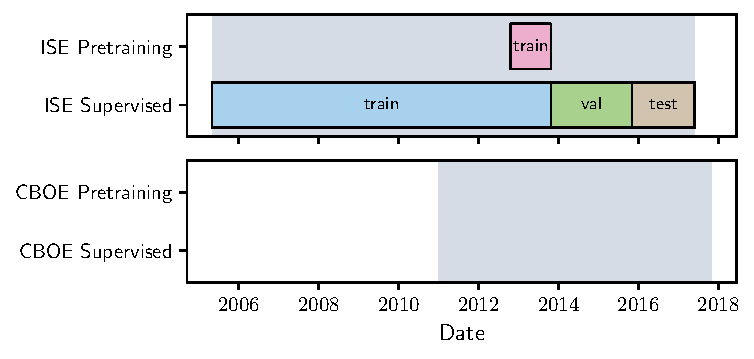
\includegraphics{train-test-split.pdf}
    \caption[Training scheme on \glsentryshort{ISE} and \glsentryshort{CBOE} Sample]{Training scheme on \gls{ISE} and \gls{CBOE} sample. The train and validation set are split by time. Shaded area \mysquare{viz-gray} indicates the duration for which the dataset is available. Own work.}
    \label{fig:train-test-split}
\end{figure}

Overall, we use \gls{ISE} data from 2 May 2005 to 24 October 2013 to train and data between 25 October 2013 and 5 November 2015 to validate our models. The most recent trades until 31 May 2017 to assess the generalisation error.

Models are pre-trained on unlabelled samples from the last year of the training period. Given the significantly larger number of unlabelled customer trades, the pre-training period is reduced to one year to facilitate training on the available computing resources. Within the period, we filter out trades for which true label can be inferred, to avoid overlaps with the supervised training set. This is essential for self-training, as labelled and unlabelled data are provided to the model simultaneously.

We use the \gls{CBOE} sample past 5 November 2015 as a second test set, as visualized in \cref{fig:train-test-split}. The start date ensures that leakage from the \gls{ISE} set is minimised~\footnote{The datasets contain features, such as the \gls{NBBO}, that are identical for both sets, assuming trades were executed at both exchanges simultaneously. Utilizing the full \gls{CBOE} sample could result in exaggerated performance estimates the corresponding \gls{ISE} trade is used in training.}.

Our train-test-split assumes that all subsets are drawn from the same distribution, so fitting a classifier on the training set and optimising for the validation set provides good estimates for the test set. To validate this assumption, we use adversarial validation. Specifically, we re-label all training samples with $y=-1$ and all trades of the validation set with $y=1$, train a classifier on a random subset of the composed dataset and predict class conformance. The performance is estimated using the \gls{MCC} of \textcite[][445]{matthewsComparisonPredictedObserved1975}, which ranges between $\left[-1, 1\right]$ and is insensitive to class imbalances~\footnote{Classes are imbalanced, due to the training set being three times the size of the validation set.}. Assuming train and validation samples are sampled from the same distribution, the performance estimate is near a random guess, or $\operatorname{MCC} = 0$, Depending on the feature sets, the \gls{MCC} ranges between \SI{0.00}{\percent} and \SI{99.999}{\percent} suggesting training and validation sets are approximately similar. The next section discusses techniques used in training the classifiers.

\subsection{Training and Tuning (10~p)}\label{sec:training-and-tuning}

\subsubsection{Training of Supervised
    Models (4~p)}\label{sec:training-of-supervised-models}

\subsubsection{Training of Semi-Supervised
    Models (4~p)}\label{sec:training-of-semi-supervised-models}


\subsubsection{Hyperparameter Tuning (2~p)}\label{sec:hyperparameter-tuning}

All of our machine-learning models feature a set of tunable hyperparameters. The results of previous studies, exemplary the one of \textcite[][5]{grinsztajnWhyTreebasedModels2022}, emphasize the need for tuning routines, as the test performance of the FT-Transformer and gradient-boosted trees largely fluctuates with the hyperparameter configuration. For a fair comparison, we employ an exhaustive hyperparameter search, to find a suitable hyperparameter configuration for each of our models.

\textbf{Bayesian Search}

We perform a novel Bayesian search to suggest and tune the hyperparameters automatically. In Bayesian search, a prior belief for all possible objective functions is formulated from the parameter intervals, which is then gradually refined by updating the Bayesian posterior with data from previous trials thereby approximating the likely objective function \autocite[][2]{shahriariTakingHumanOut2016}. Compared to brute-force approaches, such as grid search, unpromising search regions are omitted, resulting in more promising trials.

While different algorithmic implementations exist for Bayesian optimisation, we choose the optuna library by \textcite[][1--10]{akibaOptunaNextgenerationHyperparameter2019}, which implements the tree parzen estimator algorithm and is capable of handling both continuous and categorical hyperparameters. We maximize the accuracy of the validation set, which is also our decisive metric for evaluation (cp. \cref{sec:evaluation-metric}), and run $50$ trials per combination of the model and feature set. To compensate for varying computational costs between the classifiers, we set an additional time budget of 12 hours. The best combination of each is tested out-of-sample in \cref{sec:results}.

\textbf{Hyperparameter Space}

Our search space is reported in \cref{tab:hyperparameter-space}, which is laid out based on the recommendations in \textcites[][20]{prokhorenkovaCatBoostUnbiasedBoosting2018}[][18]{gorishniyRevisitingDeepLearning2021}[][4]{rubachevRevisitingPretrainingObjectives2022} with minor, reasoned deviations.

\begin{table}[H]
    \centering
    \caption{Hyperparameter Space of Gradient Boosting}
    \label{tab:hyperparameter-space}
    \begin{tabular}{llSSS}
        \toprule
        Parameter                    & Distribution                              & {\gls{GBM} 1}           & {\gls{GBM} 2}               & {\gls{GBM} 3}            \\ \midrule
        Depth                        & $\operatorname{UniformInt}[1,12]$         & 9                       & 10                          & 8                        \\
        Learning rate $\eta$         & $\operatorname{LogUniform}[0.001, 0.125]$ & 0.061147194180849546    & 0.12484853560495288         & 0.12484853839455994      \\
        $\ell_2$ Leaf Regularization & $\operatorname{UniformInt}[2, 30]$        & 16                      & 29                          & 17                       \\
        Random Strength              & $\operatorname{LogUniform}[1{e-}9, 10.0]$ & 0.000010476785242010688 & 0.0000000033898444462040114 & 0.0000013615032724416282 \\
        Bagging Temperature          & $\operatorname{Uniform}[0.0, 1.0]$        & 0.6538673528316611      & 0.4734183814715093          & 0.4515562770665896       \\ \midrule
        Accuracy in \%               &                                           & 64.20927249609458       & 75.03173105450845           & 76.98607312092097        \\ \bottomrule
    \end{tabular}
\end{table}

For gradient boosting we raise the border count to $256$, which increases the number of split candidates per feature through a finer quantization, Expectedly, accuracy increases at the cost of computational efficiency. The size of the ensemble $M$ may not be fully exhausted. Acknowledging the observations of \textcite[][14]{friedmanGreedyFunctionApproximation2001}, that the learning rate $\eta$ and the size of the ensemble have a strong interdependence, we only tune the learning rate and stop adding new trees to the ensemble, once the validation accuracy decreases for consecutive $100$ steps.

The hyperparameter search for the FT-Transformer is identical to \textcite[][18]{gorishniyRevisitingDeepLearning2021} (variant (b)). From preliminary tests, we observed that the use of a learning rate schedule with a short learning rate warm-up phase both stabilizes training and improves accuracy as derived in \cref{sec:training-of-supervised-models}. Their constant learning rate and our decayed learning rate may thus not be entirely comparable. Additionally, we implement early stopping and halt training after $15$ consecutive decreases in validation accuracy, affecting the effective number of epochs. Both techniques have not been used by the original authors to provide a conservative baseline, for the sake of a fair comparison in our work, both techniques should be used.

\textbf{Solutions For Gradient Boosting}

\begin{figure}[!b]
    \subfloat[Hyperparameter Search Space of \gls{GBM} With Feature Set 1\label{fig:ise-gbm-hyperparam-classical}]{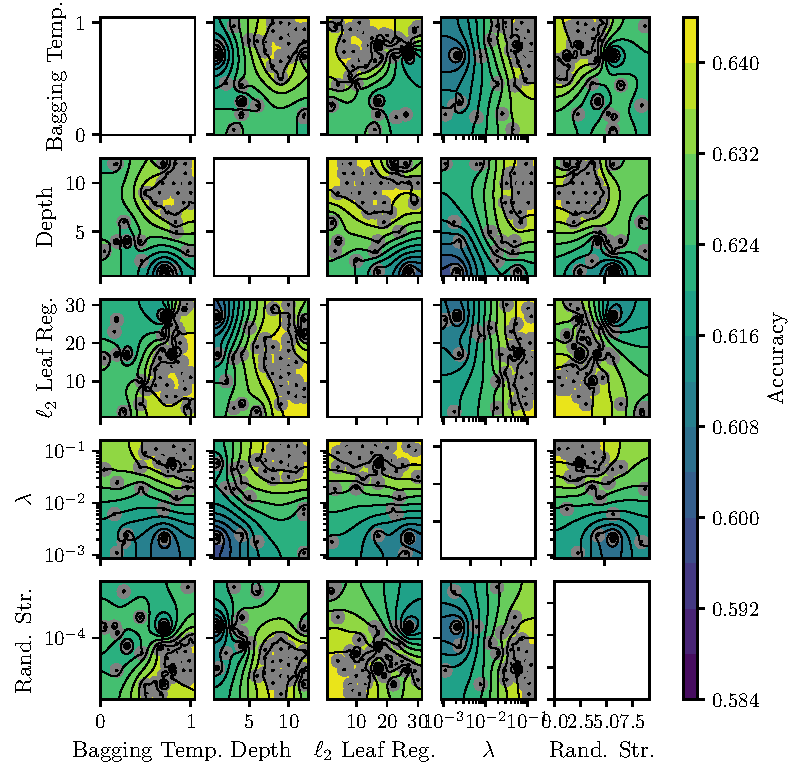
\includegraphics[ width=0.7\linewidth]{17malsep-hyperparam-search-space.pdf}}
    \vfill
    \subfloat[Hyperparameter Search Space of \gls{GBM} With Feature Set 2\label{fig:ise-gbm-hyperparam-classical-size}]{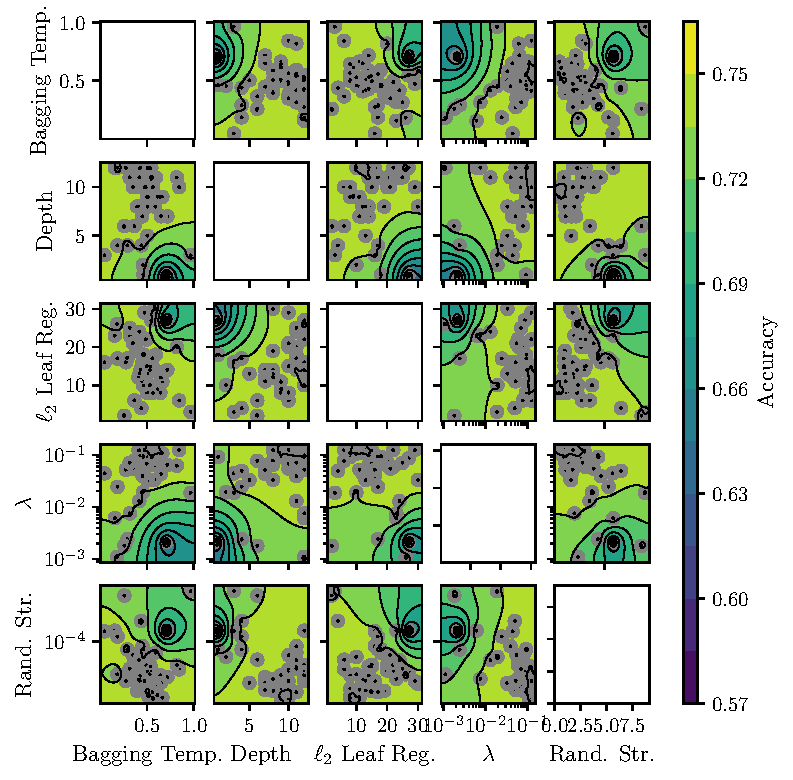
\includegraphics[ width=0.7\linewidth]{3laathab-hyperparam-search-space.pdf}}
\end{figure}

\clearpage

\begin{figure}[ht]
    \addtocounter{figure}{-1}
    \subfloat[Hyperparameter Search Space of \gls{GBM} With Feature Set 3\label{fig:ise-gbm-hyperparam-ml}]{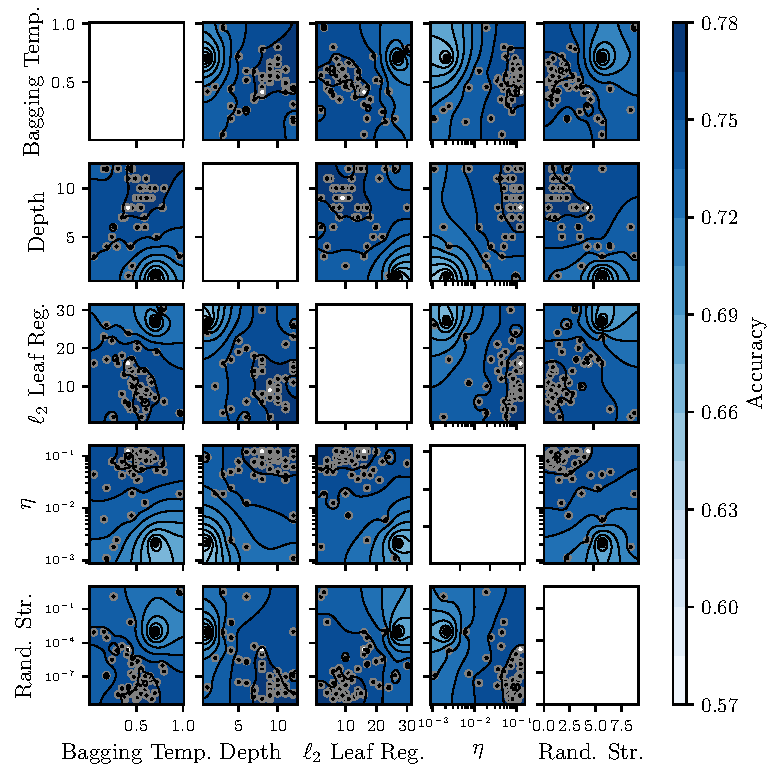
\includegraphics[ width=0.7\linewidth]{2a9iqsn0-hyperparam-search-space.pdf}}
    \caption[]{Hyperparameter Search Space of \gls{GBM} on \gls{ISE} Validation Set}
    \label{fig:ise-gbm-hyperparam}
\end{figure}
% https://wandb.ai/fbv/thesis/runs/17malsep?workspace=user-karelze
\cref{fig:ise-gbm-hyperparam-classical} visualizes the hyperparameter search space of the \gls{GBM} on the \gls{ISE} dataset with classical features. We can derive several observations from it. First, hyperparameter tuning has a significant impact on the prediction, as the validation accuracy varies between \SI{58.42}{\percent} and \SI{64.35}{\percent} for different trials. Second, the best hyperparameter combination, marked with \bestcircle, lies off-the-borders surrounded by other promising trials, indicated by the contours, from which we can conclude, that the found solution is a stable and reasonable choice for further analysis.

% https://wandb.ai/fbv/thesis/runs/3laathab?workspace=user-karelze
In \cref{fig:ise-gbm-hyperparam-classical-size} we repeat the analysis for \gls{GBM} trained on classical-size features. The loss surface is smooth with large connected regions. As the best solution achieving \SI{75.04}{\percent} accuracy lies within a splayed region of dense sampling, it is a good choice for further analysis. Consistent with the loss surface of \cref{fig:ise-gbm-hyperparam-classical}, the trees are grown to the maximum depth and a high learning rate, indicating the need for complex ensemble members highly corrective to previous predictions. Part of this could be due to the low signal-to-noise ratio in financial data.

% https://wandb.ai/fbv/thesis/runs/2a9iqsn0?workspace=user-karelze
The loss surface of the \gls{GBM} trained on the feature set including option features is the least fragmented. While the validation accuracy of the best combinations improves significantly to \SI{76.98}{\percent}, worst trials even underperform these of smaller feature sets. Based on this observation we conjecture, that more data does not per se improve the model and that models require a thoughtful tuning procedure. By this means, our conclusion contradicts the one of \textcite[][14]{ronenMachineLearningTrade2022}, who find no advantage in tuning tree-based ensembles.

% #     ("semi-classical", "3dtuffae_CatBoostClassifier_default.cbm:v7"),
% #     ("semi-classical-size", "2vnqg1sj_CatBoostClassifier_default.cbm:v8"),

\textbf{Solutions For FT-Transformer}

(insert here)

\textbf{Solutions For Classical Rules}

Akin to selecting the machine learning classifiers, we determine our classical baselines on the \gls{ISE} validation set. This prevents \gls{overfitting} the test set and maintains consistency between both paradigms. For the same reason, baselines are kept constant in the transfer setting on the \gls{CBOE} sample. Entirely for reference, we also report accuracies of the tick rule, quote rule, and \gls{LR} algorithm, due to their widespread adoption in literature.

\begin{table}[H]
    \centering
    \caption[Accuracies of Classical Trade Classification Rule on \glsentryshort{ISE} Validation Set]{Accuracies of Classical Trade Classification Rule on \gls{ISE} Validation Set}
    \label{tab:ise-classical-hyperparam-classical-size}
    \begin{table}
\centering
\caption[short-hyperparam-classical-ise_classical_supervised_val]{long-hyperparam-classical-ise_classical_supervised_val}
\label{tab:hyperparam-classical-ise_classical_supervised_val}
\begin{tabular}{lS}
\toprule
{} & {1} \\
{0} & {} \\
\midrule
trade_size(ex)->quote(best)->quote(ex)->depth(best)->depth(ex)->rev_tick(all) & 0.688359 \\
trade_size(ex)->quote(best)->quote(ex) & 0.683255 \\
trade_size(ex)->rev_lr(best) & 0.681468 \\
quote(best)->quote(ex) & 0.586736 \\
rev_lr(best)->rev_lr(ex) & 0.586463 \\
rev_lr(best) & 0.586426 \\
lr(best)->lr(ex) & 0.585902 \\
lr(best) & 0.585895 \\
quote(best) & 0.585451 \\
quote(ex)->quote(best) & 0.578577 \\
rev_lr(ex)->rev_lr(best) & 0.576739 \\
rev_lr(ex) & 0.576446 \\
lr(ex)->lr(best) & 0.575586 \\
lr(ex) & 0.575541 \\
quote(ex) & 0.575112 \\
rev_clnv(best)->rev_clnv(ex) & 0.565991 \\
rev_clnv(best) & 0.565935 \\
clnv(best)->clnv(ex) & 0.563454 \\
clnv(best) & 0.563415 \\
rev_clnv(ex)->rev_clnv(best) & 0.554454 \\
rev_clnv(ex) & 0.553904 \\
clnv(ex)->clnv(best) & 0.552497 \\
clnv(ex) & 0.552333 \\
rev_emo(best)->rev_emo(ex) & 0.548279 \\
rev_emo(best) & 0.548209 \\
emo(best)->emo(ex) & 0.548162 \\
emo(best) & 0.548136 \\
tick(all) & 0.545442 \\
tick(all)->tick(ex) & 0.545350 \\
rev_tick(all) & 0.544050 \\
rev_tick(all)->rev_tick(ex) & 0.543967 \\
emo(ex)->emo(best) & 0.537296 \\
emo(ex) & 0.537163 \\
rev_emo(ex)->rev_emo(best) & 0.537000 \\
rev_emo(ex) & 0.536375 \\
tick(ex)->tick(all) & 0.509756 \\
rev_tick(ex)->rev_tick(all) & 0.509436 \\
tick(ex) & 0.505518 \\
rev_tick(ex) & 0.503026 \\
\bottomrule
\end{tabular}
\end{table}

\end{table}

Optimizing hybrids of trade classification rules through Bayesian search is theoretically feasible, but we found no outperformance over hybrid rules already reported in literature \footnote{We performed a Bayesian search with $50$ trials for trade classification rules, stacking up to five rules. Experiment available under: \url{https://wandb.ai/fbv/thesis}.}. Thus, \cref{tab:ise-classical-hyperparam-classical-size} reports the accuracies of common trade classification rules on the \gls{ISE} validation set. The tick test applied to trade prices at the trading venue performs worst with an accuracy below a random guess. Against this backdrop, we estimate all hybrid rules involving the tick rule over all exchanges ($\operatorname{tick}_{\mathrm{all}}$). From all classical rules, a double-combination of the quote rule ($\operatorname{quote}_{\mathrm{nbbo}} \to \operatorname{quote}_{\mathrm{ex}}$), where the quote rule first applied to the \gls{NBBO} and then to quotes of the \gls{ISE}, performs best. The rule can be estimated using features from feature set one, which qualifies it as a benchmark. Also, it is commonly used in the literature, as previously by \textcite[][]{muravyevOptionsTradingCosts2020}.

By extension, we also estimate rule combinations involving overrides from the trade size rule ($\operatorname{tsize}$) and the depth rule ($\operatorname{depth}$) on the top-performing baselines of feature set one. Consistent with the recommendation of \textcite[][14]{grauerOptionTradeClassification2022}, we find that a deep stack of the $\operatorname{tsize}_{\mathrm{ex}} \to \operatorname{quote}_{\mathrm{nbbo}} \to \operatorname{quote}_{\mathrm{ex}} \to \operatorname{depth}_{\mathrm{nbbo}} \to \operatorname{depth}_{\mathrm{ex}} \to \operatorname{rtick}_{\mathrm{all}}$ achieves the highest validation accuracy. For brevity, we refer to this specific combination as the \gls{GSUH} method. Much of the performance gains are owed to the trade size and depth rules, which reduce the dependence on the reverse tick test as a last resort and provide overrides for trades at the quotes, improving validation accuracy to \SI{68.8359}{\percent}. Due to the extended use of the quoted sizes and trade sizes, it is our benchmark for the second feature set.

In absence of other baselines, we repeatedly compare against \gls{GSUH} method as a baseline for the third feature set, even if it doesn't involve option-specific features.

In the direct comparison between the validation accuracies of classical rules and our classifiers, the validation accuracies of classical rules considerably underperform the learned classifier. \cref{sec:results} discusses if the results hold for the test sets. But before we do so, we present the metrics used
for evaluation.

\subsection{Evaluation}\label{sec:evaluation}

Subsequent sub-chapters discusses metrics for evaluation and measures to retrieve feature importance estimates from the estimators.

\subsubsection{Evaluation Metric}\label{sec:evaluation-metric}

Our goal is to maximize the number of trades, where the predicted trade initiator matches the true trade initiator. We assess the quality of our model’s prediction in terms of \emph{accuracy}, which can be stated as:
\begin{equation}
    % \operatorname{accuracy} \colon \mathbb{R}^{N} \times \mathbb{R}^{N} \to  \left[0, 1\right], \quad 
    \operatorname{accuracy}(\mathbf{y}, \widehat{\mathbf{y}}) = 1 - \frac{1}{N}\sum_{i=1}^{N} \operatorname{L}_{\mathrm{0-1}}(\mathbf{y}_i, \widehat{\mathbf{y}}_i),
\end{equation}
where $\operatorname{L}_{\mathrm{0-1}}(\cdot)$ is the 0-1-loss given by:
\begin{equation}
    % \operatorname{L}_{0-1} \colon \mathcal{Y} \times \mathcal{Y} \to \left[0, 1\right], \quad 
    \operatorname{L}_{\mathrm{0-1}}(y, \hat{y}) = \mathbb{I}\left(y\neq \hat{y}\right).
\end{equation}

Intuitively, from the 0-1-loss we obtain the error rate on the dataset, as for every misclassified trade we count a loss of one and normalize by the number of samples $N$, which gives the normalized 0-1-loss. Notably, the loss is the same for false positives and negatives.

Our datasets are approximately balanced and buyer-initiated trades predicted as seller-initiated and vice versa have similar associated costs, which makes accuracy an ideal choice as a performance metric~\footnote{The \gls{ISE} test set consists of \SI{48.5973}{\percent} of buy trades and \SI{46.1278}{\percent} of the \gls{CBOE} test set are buy trades.}. As the 0-1-loss and in consequence, the accuracy is not differentiable, it cannot be used in optimisation, but as an early stopping criterion to halt training or as an optimisation target in the hyperparameter search. We report the accuracy of the test sets.

\subsubsection{Feature Importance
    Measure}\label{sec:feature-importance-measure}

Naturally, one would like to obtain insights into how the models arrived at the prediction and identify features relevant for the prediction. Both aspects can be subsumed under the term \emph{interpretability}. Following, \textcite[][4]{liptonMythosModelInterpretability2017} interpretability can be reached through model transparency or post-hoc interpretability methods. Transparent models provide interpretability through a transparent mechanism in the model, whereas post-hoc methods extract information from the already learned model \autocite[][4--5]{liptonMythosModelInterpretability2017}.

Classical trade classification algorithms, as a rule-based classifier, are transparent with an easily understandable decision process and thus provide interpretability \autocite[][91]{barredoarrietaExplainableArtificialIntelligence2020}. Interpretability, however, decreases for deep, stacked combinations involving a large feature count, when interactions between base rules become more complex and the effect of a single feature on the final prediction more challenging to interpret.

The machine-learning classifiers, studied in this work, can be deemed a black box model \autocite[][90]{barredoarrietaExplainableArtificialIntelligence2020}. Due to the sheer size of the network or ensemble, interpretability through transparency is impacted. Albeit, the attention mechanism of Transformers provides some interpretability through the attention mechanism,  interpretability across all classifiers can only be reached through a \emph{model-agnostic, post-hoc interpretability techniques}. Thereby, our goal is to identify features that are important for the \emph{correct prediction}. This is fundamentally different from methods like standard \gls{SHAP}, that attribute \emph{any} prediction to the input features \autocite[][??]{chenTrueModelTrue2020}.

Many model-agnostic methods are based on randomly permuting feature values. In this work, we specifically consider the variants \emph{permutation feature importance} \autocite[][23--24]{breimanRandomForests2001} and partial-dependence plots \autocite[][26--28]{friedmanGreedyFunctionApproximation2001}. Both serve a complementary purpose. Permutation feature importance derives the feature importance from the change in predictive accuracy before and after permuting a feature randomly, whereas partial dependence plots visualize the average change in prediction, if feature values are altered. These are widely adopted and computationally efficient.

\textbf{Random Feature Permutation}

Random feature permutation is easy to interpret by the virtue of being computationally efficient and model-agnostic. Like other feature importance measures, including \gls{SHAP}, it assumes independence between features \autocite[][2]{aasExplainingIndividualPredictions2021}.

The importance measure was originally proposed by \textcite[][23--24]{breimanRandomForests2001} for random forests and has later been extended by \textcite[][??]{fisherAllModelsAre} into a model-agnostic feature importance measure.

Random feature permutation derives the feature importance from the mean decrease in accuracy before and after permuting a feature randomly. Expectedly, permuting features break the association with the target. Thus, the permutation of important features leads to a sharp decrease in accuracy, whereas unimportant features leave the accuracy unaffected.

Given our feature matrix $\mathbf{X}$, we can define a second permuted version, $\mathbf{X}^{\pi,j}$, where the $j$-th feature is randomly permuted by $\pi$. Using $L(y_i, h(\mathbf{x}_i))$ for predicting $y_i$ from $h(\mathbf{x}_{i})$, the importance of $j$-th feature is given by:

$$
    \operatorname{VI}^{\pi}_{j} = \sum_{i=1}^{N} L(y_{i}, h(\mathbf{x}_{i}^{\pi,j})) - L(y_{i}, h(\mathbf{x}_{i})),
$$
which is the increase in loss, i.e., accuracy, before and after permutation \textcite[][82]{hookerUnrestrictedPermutationForces2021}. While \textcite[][23--24]{breimanRandomForests2001} uses a single permutation, \textcite[][??]{fisherAllModelsAre} consider multiple, random permutations. By definition, random feature importance only yields global feature importances, as the measure is aggregated from all $N$ samples.

As defined above, every feature is permuted independently from other features which artificially breaks correlations between features and creates unrealistic feature combinations. Consider, for example, the apparent correlation between the ask, bid price and trade price. Permuting only the ask could result in strongly negative or extremely large spreads since the bid remains unchanged. In effect, the presence of correlated features leads to an overestimate of the importance of correlated features \autocite[][3]{stroblConditionalVariableImportance2008}.

Vice versa, can the presence of correlated features decrease the importance of the associated feature, as the feature importance is now distributed across the features, thereby underestimating the true importance of the features. This affects all features, where information is encoded redundantly, such as the bid-ask ratio.

% (footnote-for an extended discussion of substitution effects on feature importance in the financial domain see \textcite[][114--118]{lopezdepradoAdvancesFinancialMachine2018}.

To alleviate the bias from dependent, we group dependent features and estimate the feature importance on a group-level. Arranging all features in a tree-like hierarchy gives us the freedom to derive feature importances at different levels, enabling cross-comparisons between classical rules and other classifiers, as the grouping of raw and derived features makes the implementation of classical rules transparent.

% (footnote: Consider the implementation of the tick rule. Here, the implementation could use the feature price lag (ex) or calculate the price change from the trade price and price lag (ex). If not grouped, feature importances would be attributed to either the derived feature or raw features causing difficulties in comparison with machine learning classifiers, which have access to all three features simultaneously. Grouping all three features resolves this issue at the cost of interpretability.). 

Other than the classical random feature permutation, all features sharing the same parent node are permuted together. We define the following dependency structure:
(tbd)

\textbf{Partial Dependence Plots}

Related to the concept of random feature permutation are partial dependence plots by \textcite[][26--28]{friedmanGreedyFunctionApproximation2001} visualize the dependency between a single feature or multiple features and the effect on the target value as the feature value is adjusted / after marginalizing out all other features. Let $\mathbf{X}^{x,j}$ be a matrix, where the $j$-th feature value is replaced by $x$ and all other features are unaltered, partial feature dependence function:
\begin{equation}
    \operatorname{PD}_{j}(x) = \frac{1}{N} \sum_{i=1}^{N} h(\mathbf{x}^{x,j}_{i}),
\end{equation}
now gives the marginal average over all other features \autocite[][81]{hookerUnrestrictedPermutationForces2021}. By iterating over a grid of (observed) $x$, we obtain the partial dependence plot for the feature.

Like random feature permutation, partial dependence plots are a global feature importance measure, unable to capture dependencies between features and visualization is constrained to two dimensions or features at once \autocite[][p. 388]{hastietrevorElementsStatisticalLearning2009}. Despite these limitations partial dependence plots help us verify the assumed relationships in classical rules, such as the linear relationship in the tick rule, with the learned relationships in our classifier.


\textbf{Attention Maps}

In addition to permutation-based methods, Transformer-based models offer \emph{some} interpretability through their attention mechanism. In recent research a major controversy embarked around the question, of whether attention offers explanations to model predictions \autocites[cp.][150]{bastingsElephantInterpretabilityRoom2020}[][5--7]{jainAttentionNotExplanation2019}[][9]{wiegreffeAttentionNotNot2019}. The debate sparked around opposing definitions of explainability and the consistency of attention scores with other, established feature-importance measures. Our focus is less on post-hoc explainability of the model, but rather on transparency. Consistent with \textcite[][8]{wiegreffeAttentionNotNot2019} we view attention scores as a vehicle to model transparency.

Recall from our discussion on attention (cp. \cref{sec:attention}) that the attention matrix stores how much attention a token pays to each of the keys. Thus, feature attributions can be derived from attention by visualizing features to which the model is paying attention to in an attention map. While attention maps are specific to Transformers or other attention-based architectures, rendering them useless for cross-model comparisons, they give additional insights from different attention layers and attention heads of the model on a per-trade and global basis. An example is shown in \cref{fig:attention-maps}.

\begin{figure}[ht]
    \centering
    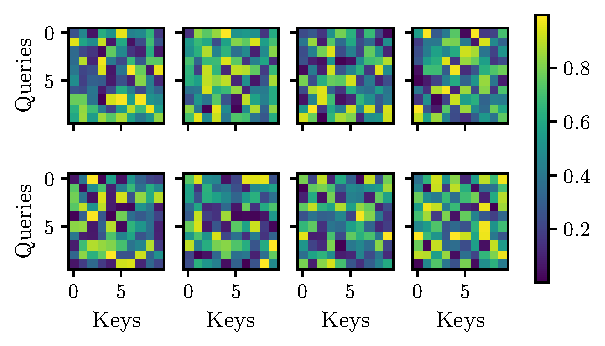
\includegraphics{attention-maps.pdf}
    \caption[Attention Maps]{Attention Maps. Own work.}
    \label{fig:attention-maps}
\end{figure}

In the tabular domain, various approaches have been investigated in the literature to obtain attention from multiple attention heads and Transformer blocks. \textcite[][18]{somepalliSaintImprovedNeural2021} and \textcite[][11]{borisovDeepNeuralNetworks2022} gather attention maps from the first attention layer only, and \textcite[][11]{borisovDeepNeuralNetworks2022} additionally obtain feature attributions by taking the diagonal of the attention matrix $\mathbf{A}$ or through column-wise summation. In contrast, \textcite[][10]{gorishniyRevisitingDeepLearning2021} leverage all attention matrices by averaging over multiple Transformer blocks, attention heads, and samples to obtain global feature attributions. Given \cref{sec:architectural-overview,sec:attention}, where we emphasized the unique role of attention heads and lower sublayers, both approaches may be myopic, as attention heads may contribute unequally to the result, or as later attention layers are neglected altogether.

While not explored systematically in the tabular domain yet, the rollout attention method of \textcite[][3]{abnarQuantifyingAttentionFlow2020} combines raw attention from multiple layers through recursive matrix multiplication with the weight matrices from attention layers below, as shown in this Equation~\footnote{Notation from adapted from \textcite[][786]{cheferTransformerInterpretabilityAttention2021}.}:
\begin{equation}
    \begin{aligned}
        \hat{\mathbf{A}}^{(l)}    & =\mathbf{I}+\mathbb{E}_h \mathbf{A}^{(l)}                                              \\
        \operatorname { rollout } & =\hat{\mathbf{A}}^{(1)} \cdot \hat{\mathbf{A}}^{(2)} \ldots\cdot\hat{\mathbf{A}}^{(L)}
    \end{aligned}
    \label{eq:attention-map-rollout}
\end{equation}

In each layer the raw attention scores $\mathbf{A}^{(l)}$ are averaged over $h$ heads, denoted by $\mathbb{E}_h$. The identity matrix $\mathbf{I}$ is added to account for the residual connections (\cref{sec:residual-connections-layer-norm}). While rollout attention considers all attention layers in the calculation of feature attributions, it does not consider a signal and attributes equal weights to all attention heads \autocite[][786]{cheferTransformerInterpretabilityAttention2021}.

In an attempt to explain the decision-making process of multi-modal Transformers, including self-attention-based Transformers, \textcite[][3]{cheferTransformerInterpretabilityAttention2021} incorporate gradients to weight the head's contribution when averaging over the heads of a layer, as shown in \cref{eq:attention-map-weighted}. Like before, all attention layers are considered.

\begin{equation}
    \begin{aligned}
        \bar{\mathbf{A}}^{(l)}   & =I+ \mathbb{E}_h\left(\left(\nabla \mathbf{A}^{(l)} \odot \mathbf{A}^{(l)}\right)^{+}\right) \\
        \operatorname {wrollout} & =\bar{\mathbf{A}}^{(1)} \cdot \bar{\mathbf{A}}^{(2)} \ldots \cdot \bar{\mathbf{A}}^{(L)}
    \end{aligned}
    \label{eq:attention-map-weighted}
\end{equation}

In this approach, the element-wise product between the gradient of the attention map $\nabla \mathbf{A}^{(l)}=\frac{\partial y_t}{\partial \mathbf{A}}$ for the model's target class $t$ and the attention map $\mathbf{A}^{(l)}$ is calculated to weight the attention head's importance. As previously suggested in \textcite[][786]{cheferTransformerInterpretabilityAttention2021}, negative contributions are eliminated to focus on the positive relevance, and the results are averaged over the heads dimension. Like all other presented approaches \cref{eq:attention-map-rollout,eq:attention-map-weighted} can be computed with a single forward pass and is therefore computationally efficient.

In absence of ground truth for the true feature attribution, we resort to attention maps using \cref{eq:attention-map-weighted}. Following prior research, feature attributions are also summed over the first attention layer or all transformer blocks. The level of agreement between attributions from attention maps and random feature permutation by calculating Spearman's rank correlation between them.

\newpage
\section{Results}\label{sec:results}


\subsection{Results of Supervised
    Models (2~p)}\label{sec:results-of-supervised-models}

\textbf{Gradient Boosting}

\textbf{FT-Transformer}

\subsection{Results of Semi-Supervised
    Models (2~p)}\label{sec:results-of-semi-supervised-models}


\textbf{Gradient-Boosting With Self-Training}

\textbf{FT-Transformer With Pretraining}

\subsection{Robustness of Results (3~p)}\label{sec:robustness-checks}

\subsection{Feature Importance (3~p)}\label{sec:feature-importance}

% \subsection{Ablation Study of Models (2~p)}\label{sec:ablation-study}

\newpage
\section{Application in Transaction Cost Estimation}\label{sec:application}

\textbf{Preliminaries}

% TODO: Add why it is important. See Stoll, Huang, Roll (zettelkasten)

Albeit the classification accuracy is a reasonable measure for comparing classifiers, one cannot immediately infer how changes in accuracy e.~g., an improvement by \SI{1}{\percent}, affect the application domains. In an attempt to make our results tangible, we apply all algorithms to estimate trading cost, a problem we previously identified to be reliant on correct trade classification (cp. \cref{sec:introduction}) and a common testing ground for trade classification rules \autocites[cp.][541]{ellisAccuracyTradeClassification2000}[][569]{finucaneDirectTestMethods2000}[][271--278]{petersonEvaluationBiasesExecution2003}[][896--897]{savickasInferringDirectionOption2003}.

One of the most widely adopted measures for trading costs is the effective spread \autocite[][112]{Piwowar_2006}. It is defined as the difference between the trade price and the fundamental value of the asset \autocite[][238--239]{bessembinderIssuesAssessingTrade2003}. Following \textcite[][238--239]{bessembinderIssuesAssessingTrade2003}, we define the \emph{nominal, effective spread} as
\begin{equation}
    S_{i,t} = 2 (P_{i,t} - V_{i,t}) D_{i,t}.
    \label{eq:effective-spread}
\end{equation}

Like before, $i$ indexes the security and $t$ the point in time. Here, $D_{i,t}$ is the trade direction, which is either $1$ for customer buy orders and $-1$ for sell orders. If the trade initiator is known, we set $D_{i,t} = y_{i,t}$ and $D_{i,t}=\hat{y}_{it}$, if inferred from a rule or classifier. As the fundamental value $V_{i,t}$ is unobserved at the time of the trade, we follow a common track in research and use the midpoint of the prevailing quotes as an observable proxy \footnote{An alternative treatment for options is discussed in \textcite[][4975--4976]{muravyevOptionsTradingCosts2020}. Our focus is on the midspread, as it is the most common proxy for the value.}. This is also a natural choice, under the assumption that, on average, the spread is symmetric and centred around the true fundamental value \autocite[][1018]{leeMarketIntegrationPrice1993}. We multiply the so-obtained half-spread by $\times 2$ to obtain the effective spread, which represents the cost for a round trip trade involving a buy and sell excluding commissions.

Apparent from \cref{eq:effective-spread}, poor estimates for the predicted trade direction, lead to an under or overestimated effective spread, and hence to a skewed trade cost estimate. Only for trades at the midspread, the predicted trade direction is irrelevant, since the effective spread is zero. By comparing the true effective spread from the estimated, we can derive the economic significance. For convenience, we also calculate the \emph{relative effective spread} as
\begin{equation}
    {PS}_{i,t} = S_{i,t} / V_{i,t}.
\end{equation}
% FIXME: check how it is defined Savickas / Finucane use midpoint, Peterson and Sirri divide by price / so does chakrabarty 2007 p. 3819?
The subsequent section estimates both the nominal and relative effective spread for our test sets, as well as the quoted spread.

\textbf{Results}

The actual and the estimated effective spreads, as well as the quoted spread, are shown in the \cref{tab:effective-spread} aggregated by mean. \textcite[][896--897]{savickasInferringDirectionOption2003} estimated the effective spreads on a subset of rules for option trades at the \gls{CBOE}, which can be compared against.

\begin{table}[H]
    \centering
    \begin{threeparttable}
    \sisetup{
        round-precision = 3, 
      }
    \begin{tabular}{llSSSS}
        \toprule
        {}                                               & {}   & \multicolumn{2}{c}{\gls{ISE}} & \multicolumn{2}{c}{\gls{CBOE}}                                 \\ \cmidrule(lr){3-4}\cmidrule(lr){5-6}
        {Classifier}                                     & {FS} & {Dollar}                      & {Relative}                     & {Dollar} & {Relative}         \\ \midrule
        \multicolumn{6}{l}{Rule-Based}                                                                                                                           \\
        \tabindent $\operatorname{tick}_{\mathrm{ex}}$   & 1    & 0.015534                      & 0.010777 \tnote{*}             & 0.014179 & 0.022880 \tnote{*} \\
        \tabindent $\operatorname{quote}_{\mathrm{ex}}$  & 1    & 0.163333                      & 0.162074 \tnote{*}             & 0.125388 & 0.142093 \tnote{*} \\
        \tabindent $\operatorname{lr}_{\mathrm{ex}}$     & 1    & 0.163333                      & 0.162074 \tnote{*}             & 0.125388 & 0.142093 \tnote{*} \\
        \tabindent $\operatorname{emo}_{\mathrm{ex}}$    & 1    & 0.046443                      & 0.084442 \tnote{*}             & 0.041138 & 0.074176 \tnote{*} \\ 
        \tabindent $\operatorname{clnv}_{\mathrm{ex}}$   & 1    & 0.116247                      & 0.132842 \tnote{*}             & 0.086715 & 0.110510 \tnote{*} \\ 
        \tabindent $\operatorname{gsu}_{\mathrm{small}}$ & 2    & 0.065670                      & 0.096277 \tnote{*}             & 0.084145 & 0.107195 \tnote{*} \\
        \tabindent $\operatorname{gsu}_{\mathrm{large}}$ & 2    & 0.016734                      & 0.044854 \tnote{*}             & 0.053114 & 0.072212 \tnote{*} \\ \midrule
        \multicolumn{6}{l}{Supervised}                                                                                                                           \\
        \tabindent \gls{GBRT}                            & 1    & 0.074294                      & 0.091619 \tnote{*}             & 0.060933 & 0.095318 \tnote{*} \\
        \tabindent \gls{GBRT}                            & 2    & 0.042556                      & 0.069838 \tnote{*}             & 0.036213 & 0.071433 \tnote{*} \\
        \tabindent \gls{GBRT}                            & 3    & 0.039437                      & 0.066473 \tnote{*}             & 0.034674 & 0.066758 \tnote{*} \\ 
        \tabindent  FT-Transformer                       & 2    & 0.030291                      & 0.065596 \tnote{*}             & 0.024942 & 0.063574 \tnote{*} \\
        \tabindent  FT-Transformer                       & 1    & 0.065871                      & 0.086339 \tnote{*}             & 0.057153 & 0.090205 \tnote{*} \\
        \tabindent  FT-Transformer                       & 3    & 0.029874                      & 0.063486 \tnote{*}             & 0.021487 & 0.057358 \tnote{*} \\ \midrule
        \multicolumn{6}{l}{Semi-Supervised}                                                                                                                      \\
        \tabindent \gls{GBRT}                            & 1    & 0.075724                      & 0.092439 \tnote{*}             & 0.065420 & 0.096814 \tnote{*} \\
        \tabindent \gls{GBRT}                            & 2    & 0.043359                      & 0.072062 \tnote{*}             & 0.039600 & 0.073760 \tnote{*} \\
        \tabindent \gls{GBRT}                            & 3    & 0.043240                      & 0.069230 \tnote{*}             & 0.037083 & 0.067946 \tnote{*} \\ 
        \tabindent  FT-Transformer                       & 1    &                               & \tnote{*}                      &          & \tnote{*}          \\
        \tabindent  FT-Transformer                       & 2    &                               & \tnote{*}                      &          & \tnote{*}          \\
        \tabindent  FT-Transformer                       & 3    &                               & \tnote{*}                      &          & \tnote{*}          \\ \midrule
        True Effective Spread                            &      & 0.004926                      & 0.037159                       & 0.012219 & 0.025122           \\ \bottomrule
        % Quoted Spread                                    &      &                                                   &                                                    &          &                 \\ \bottomrule
    \end{tabular}
    \begin{tablenotes}\footnotesize
        \item[*] $p \leq 0.01$.
    \end{tablenotes}
\end{threeparttable}
    \caption{Effective Spreads Estimates of Trade Classification Rules and Classifiers}
    \label{tab:effective-spread}
\end{table}

Following \textcite[][12]{theissenTestAccuracyLee2000} a Wilcoxon test is conducted to assess if the medians of the estimated, effective spread and the true effective spread are equal. The null hypothesis of equal medians is rejected for $p \leq 0.01$.


% TODO: Discuss results. See Zettelkasten.

\newpage
\section{Discussion (3~p)}\label{sec:discussion}

\newpage
\section{Conclusion (2~p)}\label{sec:conclusion}

\newpage
\section{Outlook (0.5~p=67.5~p)}\label{sec:outlook}



% Bibliography
\newpage
\printbibliography

% Glossary
\newpage
\printglossary[type=main,title=Glossary,style=altlist]


% Appendix
\newpage
\appendix % Enumerates appendix with letters.
\section{Appendix}

\begin{table}[H]
    \centering
    \begin{threeparttable}
    \begin{tabular}{@{}lllllll@{}}
        \toprule
        Feature Name            & Definition                                                                                       & Origin               & FS 1 & FS 2 & FS 3 & Transform     \\ \midrule
        trade price             & $P_{i, t}$                                                                                       & tick rule            & x    & x    & x    & $\log(\cdot)$ \\
        price lag (ex)          & $P_{i, t-1}^{\text{ex}}$\tnote{*}                                                                & tick rule            & x    & x    & x    & $\log(\cdot)$ \\
        price lag (all)         & $P_{i, t-1}^{\text{all}}$\tnote{*}                                                               & tick rule            & x    & x    & x    & $\log(\cdot)$ \\
        price change lag (ex)   & $P_{i, t-1}^{\text{ex}}/P_{i, t}^{\text{ex}}$\tnote{*}                                           & tick rule            & x    & x    & x    &               \\
        price change lag (all)  & $P_{i, t-1}^{\text{all}}/P_{i, t}^{\text{all}}$\tnote{*}                                         & tick rule            & x    & x    & x    &               \\
        priced lead (ex)        & $P_{i, t+1}^{\text{ex}}$\tnote{*}                                                                & rev. tick rule       & x    & x    & x    & $\log(\cdot)$ \\
        price lead (all)        & $P_{i, t+1}^{\text{all}}$\tnote{*}                                                               & rev. tick rule       & x    & x    & x    & $\log(\cdot)$ \\
        price change lead (ex)  & $P_{i, t}^{\text{ex}}/P_{i, t+1}^{\text{ex}}$\tnote{*}                                           & rev. tick rule       & x    & x    & x    &               \\
        price change lead (all) & $P_{i, t}^{\text{all}}/P_{i, t+1}^{\text{all}}$\tnote{*}                                         & rev. tick rule       & x    & x    & x    &               \\
        bid (all)               & $B_{i, t}^{\text{all}}$                                                                          & quote rule           & x    & x    & x    & $\log(\cdot)$ \\
        bid (ex)                & $B_{i, t}^{\text{ex}}$                                                                           & quote rule           & x    & x    & x    & $\log(\cdot)$ \\
        ask (all)               & $A_{i, t}^{\text{all}}$                                                                          & quote rule           & x    & x    & x    & $\log(\cdot)$ \\
        ask (ex)                & $A_{i, t}^{\text{all}}$                                                                          & quote rule           & x    & x    & x    & $\log(\cdot)$ \\
        prox. to quotes (ex)    & $\left(P_{i, t}^{\text{ex}}- M_{i, t}^{\text{ex}}\right) / \tfrac{1}{2} S_{i, t}^{\text{ex}}$    & \gls{EMO}/\gls{CLNV} & x    & x    & x    &               \\
        prox. to quotes (all)   & $\left(P_{i, t}^{\text{all}}- M_{i, t}^{\text{all}}\right) / \tfrac{1}{2} S_{i, t}^{\text{all}}$ & \gls{EMO}/\gls{CLNV} & x    & x    & x    &               \\
        bid ask size ratio (ex) & $\tilde{B}_{i, t}^{\text{ex}}/\tilde{A}_{i, t}^{\text{ex}}$                                      & depth rule           &      & x    & x    &               \\
        bid size (ex)           & $\tilde{B}_{i, t}^{\text{ex}}$                                                                   & depth rule           &      & x    & x    &               \\
        ask size (ex)           & $\tilde{A}_{i, t}^{\text{ex}}$                                                                   & depth rule           &      & x    & x    &               \\
        rel. bid size (ex)      & $\tilde{B}_{i, t}^{\text{ex}}/\tilde{P}_{i, t}^{\text{ex}}$                                      & trade size rule      &      & x    & x    &               \\
        rel. ask size (ex)      & $\tilde{A}_{i, t}^{\text{ex}}/\tilde{P}_{i, t}^{\text{ex}}$                                      & trade size rule      &      & x    & x    &               \\
        trade size              & $\tilde{P}_{i, t}$                                                                               & trade size rule      &      & x    & x    &               \\
        strike price            &                                                                                                  & option               &      &      & x    & $\log(\cdot)$ \\
        volume option series    &                                                                                                  & option               &      &      & x    & $\log(\cdot)$ \\
        root                    &                                                                                                  & option               &      &      & x    & binarize      \\
        time to maturity        &                                                                                                  & option               &      &      & x    &               \\
        moneyness               &                                                                                                  & option               &      &      & x    &               \\
        option type             &                                                                                                  & option               &      &      & x    & binarize      \\
        issue type              &                                                                                                  & option               &      &      & x    & binarize      \\ \bottomrule
    \end{tabular}
    \begin{tablenotes}\footnotesize
        \item[*] Notation assumes, that the previous or next trade price is distinguishable.
    \end{tablenotes}
\end{threeparttable}
    \caption[Feature Set Definition]{Feature Set Definition}
    \label{tab:feature-set-definition}
\end{table}

\end{document}